\documentclass[11pt,a4paper]{ivoa}
\input tthdefs

\usepackage{array}
\usepackage{tabulary}  % for nicer tables
\usepackage{calc}
\usepackage{placeins}
\usepackage{enumitem}
\setlength\extrarowheight{2pt}

\newcolumntype{L}{>{\centering\arraybackslash}m{3cm}}
\title{MANGO: A Model for ANnotating Generic Objects}

% see ivoatexDoc for what group names to use here
\ivoagroup{DM}


% mireille commands
% borrowed from Prov WD - Kristin - own definitions
\definecolor{todocolor}{rgb}{1,1,0.8}
\definecolor{darkred}{rgb}{0.6,0,0}
\definecolor{rose}{rgb}{1.0,0.88,0.88}
\definecolor{darkgrey}{rgb}{0.35,0.35,0.35}
%\newcommand{\TODO}[1]{%
%    \noindent%
%    \textcolor{todocolor}{\sffamily [\textbf{TODO:} #1]}%
%}

\newcommand{\TODO}[1]{%
    \noindent%
    \colorbox{todocolor}{%
            \parbox{0.85\linewidth}{\sffamily \textbf{TODO:}\\
            #1}
    }%
    \vspace{2pt}

}

\newcommand{\note}[1]{%
    \noindent%
    \textcolor{darkgrey}{{\sffamily Note:} \emph{#1}}%
}

\newcommand{\comment}[1]{%
    \noindent%
    \textcolor{red}{{\sffamily Comment:} \emph{#1}}%
}


\author{François Bonnarel}
\author{Gilles Landais}
\author{Laurent Michel}
\author{Jesus Salgado}
\author{Mireille Louys}
\author{Marco Molinaro}

\editor{Laurent Michel}

\previousversion{This is the first public release}

\begin{document}

\begin{abstract}

The MANGO data model proposes a flexible way to expose data related to astronomical source objects 
in an interoperable way.
It takes into account the huge diversity of source data in terms of feature description, format and usage.
The MANGO model deals with catalog entries, corresponding to astronomical sources or detections of those and represent them as a MANGO Object class.  
It attaches identifiers on the "MANGO object" class and associates to each one a flexible 
set of properties (e.g. observed physical quantities). It also offers to link other information like detection status, quality annotation, preview images, etc.
Properties may be expressed as several columns of a data table.
Additional data products (e.g. spectra, time series) may be bound to the source entry to contribute to the science analysis and enhance data understanding.
MANGO object properties are built upon classes or extended classes of the IVOA Measure
and Coordinates data models. It also reuses PhotDM and proposes its own classes for the quantities 
that are not covered by the imported models.
Associated data can be provided as simple URLs or VO service endpoints.
The roles of both properties and associated data are qualified by semantic tags to provide rich context. 

\end{abstract}


\section*{Acknowledgments}

We would like to thank all people at INAF, CDS, CFA, ESAC, etc.  who took the time to present their own use cases on which the model has been built.
We would also like to thank all the people having tested MANGO on their own data.

\section*{Model Name}
This model was initially named with a very explicit but hard to remember acronym, \texttt{CAB-MSD}
standing for Component and Association Based Model for Source Data.
We decided later to rename it \texttt{MANGO} with reference to the inside out MANGO
picture used to introduce the model in Groningen. 
As the tradition requires that such unexpected names are acronyms,
let's assume that \texttt{MANGO} stands for
Metadata ANnotation for Generic Objects (in astronomy).


\section*{Conformance-related definitions}

The words ``MUST'', ``SHALL'', ``SHOULD'', ``MAY'', ``RECOMMENDED'', and
``OPTIONAL'' (in upper or lower case) used in this document are to be
interpreted as described in IETF standard RFC2119 \citep{std:RFC2119}.

The \emph{Virtual Observatory (VO)} is a
general term for a collection of federated resources that can be used
to conduct astronomical research, education, and outreach.
The \href{http://www.ivoa.net}{International
Virtual Observatory Alliance (IVOA)} is a global
collaboration of separately funded projects to develop standards and
infrastructure that enable VO applications.


\section{Introduction}

Modeling data collected to study astronomical source objects has been a long term concern for the 
DM working group and more generally for the IVOA.
In the past years, there were some proposals to design a global model for sources \citep{wd:jesusdm}
as well as for catalogs \citep{wd:catalog}.
Other proposals, more model-agnostic, were focused on the data annotation in VOTables
\citep{note:stcvot} \citep{note:seb}.
In this case the goal was no longer to design a source model but to provide a complete description of
individual quantities (positions, velocity, fluxes, magnitudes…).
None of these proposals have come to completion due to the complexity of the task.

The source DM issue resurfaced at the spring 2018 Interop in Victoria during an hands-on session
focusing on the tools available to work with VO data models and especially with VO-DML.
The goal of this session was to annotate data from different origins in order to make them
interoperable with each other.
The main concern expressed during this session was not much related to the tools themselves
but indeed to the lack of models for sources.
This is a paradox in the VO world: source data which represent the basic building
blocks of astronomers' work, is not modelled.
This paradox can be explained by the fact that the observation of source objects is multi-faceted.
In a general way, the way features for source data are described and organised depends on
the targeted science case.
Principal investigators and archive designers set up the data profile and structure it according
to this goal which varies from one project to another.
Therefore this diversity cannot be served by a single static data model describing a source
item for all possible cases.
Having a global source model would lead to a very complex solution not usable in practice.

This standard proposes to overcome this paradox and presents a template model gathering independent
components from VO existing models embedded on demand in a container.

MANGO is not designed to describe what a source is but to help clients to discover and to understand
the quantities available for a particular source instance.
VOtable data mapped on MANGO with Mivot (2023ivoa.spec.0620M) annotations can be consumed quantity 
par quantity instead of column per column.
The way complex quantities are built is  described by MANGO but no longer by the clients.

\subsection{Role within the VO Architecture}

\begin{figure}
\centering

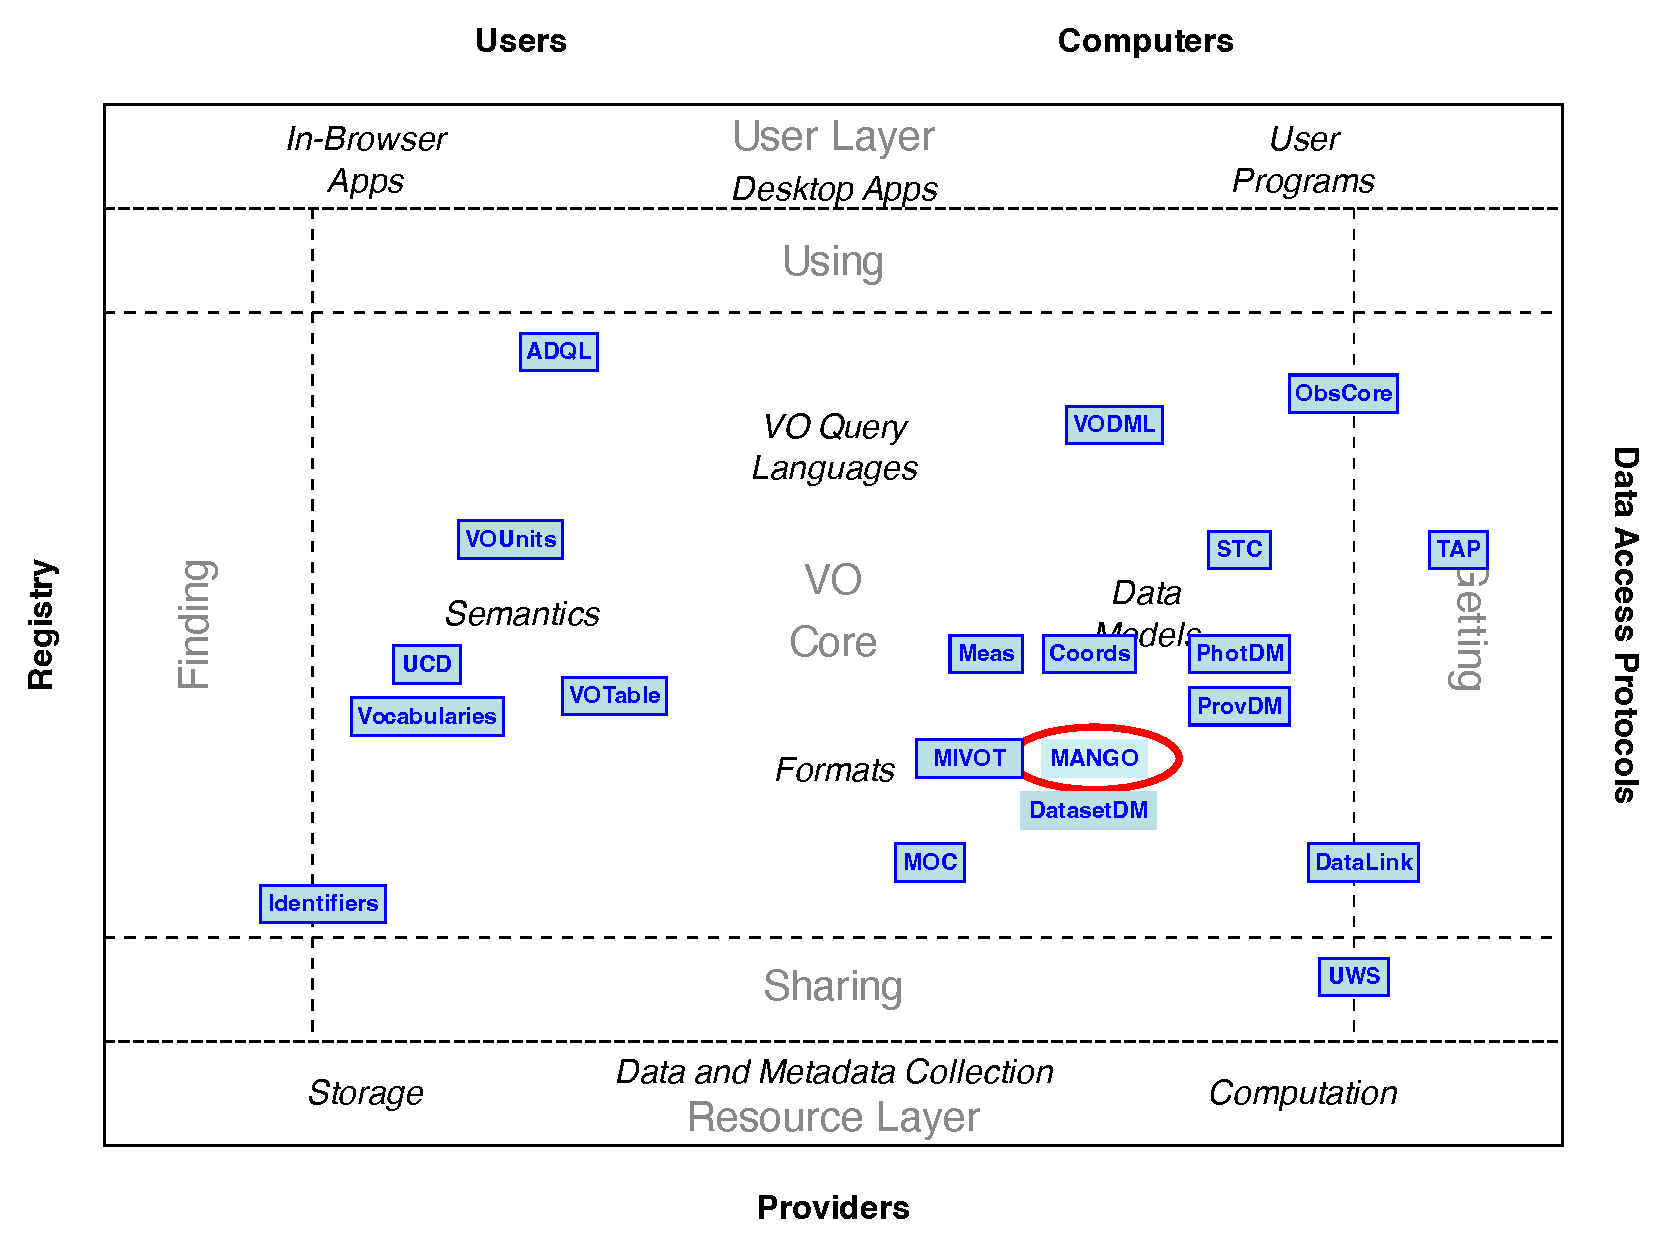
\includegraphics[width=0.9\textwidth]{role_diagram.pdf}
\caption{Architecture diagram for this document}
\label{fig:archdiag}
\end{figure}

Fig.~\ref{fig:archdiag} shows the role this document plays within the
IVOA architecture \citep{2010ivoa.rept.1123A}.


\section{Representing observed astronomical objects : Use Cases and  Requirements}

\subsection{Use Cases}

The main purpose of MANGO is to add an upper description level to the tabular data of query responses.
MANGO is not designed to replace the meta-data already present in query responses, 

Uses-cases have been collected since 2019 from representatives of various astronomical 
missions, archive designers and tools developers.
The contribution was totally open. This gave a good picture of the needs but we do not pretend 
that everything will be supported by this first version.
All the use-cases summarized below are detailed in appendix.

\subsubsection{Gaia}
Gaia mission is producing the largest and more precise 3D map of our galaxy.
Gaia core solution is able to solve the astrometric solution of more than 1
billion sources by complex models and algorithms \citep{2012A&A...538A..78L}.
Using a minimisation problem approach, different detections identified on
different scans can be associated to the same astronomical source. Some of the
properties would be direct measurements on single scans (e.g. positions or
magnitudes). Also other properties like radial velocity (measured in redshift
units) are also obtained at integration time of the scans.

A non-exhaustive list of properties required for Gaia use cases would be composed
of:

\begin{itemize}[noitemsep,topsep=0pt,parsep=0pt,partopsep=0pt]
    \item identifier
    \item sky reference position
    \item proper motion
    \item parallax and distance

    \item source extension
    \item radial velocity
    \item redshift
    \item photometry
    \item date of detection
    \item correlation
    \item multiple detection
\end{itemize}

\subsubsection{Euclid}
Euclid telescope has been designed to unveil some of the questions about the
dark Universe, including dark matter and dark energy, what would include, e.g.
quite accurate measurements of the expansion of the Universe.

Euclid will mainly observe extragalactic objects providing, e.g. information
of the shapes of galaxies, gravitational lensing,  baryon acoustic oscillations
and distances to galaxies using spectroscopic data.

For this mission, and apart from the common metadata provided for extra galactic
sources into astronomical catalogues, a good support for object taxonomy and
shapes of objects will be required. As known due to general relativity effects,
shapes far galaxies could be deformed due to gravitational lensing effects,
producing convergence (visual displacements on the position) and rear (deformation
of the shape) effects. All these metadata should be ready for annotations and,
also, correlated to theoretical or real metadata in other datasets.

Finally, crossmatch information with other catalogues will be of crucial interest
as data from other satellites and, more importantly, from ground based
observatories will be combined with Euclid data to produce consistent scientific
datasets.

\begin{itemize}[noitemsep,topsep=0pt,parsep=0pt,partopsep=0pt]
    \item identifier
    \item sky position
    \item correlation with other catalogues
    \item photometry (ground + satellite )
    \item morphology class
    \item redshift
    \item photometric redshift
\end{itemize}
From the above contributions we can issue a list of use cases that lead the MANGO design: 

\subsubsection{Exoplanets}
Annotation of (exo-)planetary records in catalogues requires some
specific metadata or model.

The use cases identified requires the following metadata:
\begin{itemize}[noitemsep,topsep=0pt,parsep=0pt,partopsep=0pt]
	\item the degree of confidence in the detection: exoplanets candidates
w.r.t. confirmed ones, plus last update of the record content ;
	\item the method used in the discovery (since it affects the available
stellar system description parameters);
	\item a set of stellar host characteristics (besides sky coordinates):
activity, mass, type,
metallicity, age, some systemic values, like the global RV (radial
velocity) of the system, and so on;
	\item (exo-)planet parameters, like mass, orbital period, orbit's
eccentricity, RV semi-amplitude, time at periastron (for RV detections)
or central transit time (for transit method), longitude of periastron,
and so on.
\end{itemize}
 
 
\subsubsection{Morphologically Complex Structures}
The ViaLactea Knowledge Base (VLKB, see \cite{2016SPIE.9913E..0HM}) is a set of data
resources and services built up to study the star formation regions and
processes in the Milky Way. Besides 2-D images and 3-D radial velocity
cubes, the VLKB exposes a bunch of source catalogues.
A model that supports description of such catalogues will need a
way to describe sources with:
\begin{itemize}[noitemsep,topsep=0pt,parsep=0pt,partopsep=0pt]
	\item non-point-like positions;
	\item extended complex area, possibly as multiple detached areas;
	\item aggregation of sub-parts (that can be heterogeneous).
\end{itemize}

\subsubsection{Chandra Archive}
The Chandra Source Catalog(CSC) is the definitive catalog of serendipitous X-ray sources identified in
publicly released imaging observations obtained by NASA’s ChandraX-ray Observatory (CXO).

The catalog itself consists of approximately 1,700 columns covering properties at the 
individual observation and stacked analysis levels.
Table \ref{tab:chandra_properties} summarizes some of the basic catalog properties derived
from standard CSCView queries. 

\begin{table}[ht!]
  \tiny
  \begin{tabular}{|p{0.4cm}p{10.0cm}|}
    \hline
    \multicolumn{2}{|l|}{\textbf{Per Source:}} \\
    & \texttt{ Source name } \\
    & \texttt{ Source position and position errors } \\
    & \texttt{ Significance of the source (signal to noise) } \\
    & \texttt{ Likelihood of the source  (True, False, or Marginal detection) } \\
    & \texttt{ Source extent flag } \\
    & \texttt{ Variability flag } \\
    & \texttt{ Spectral variability flag } \\
    & \texttt{ Fluxes and flux errors in ACIS bands b, h, m, s, u } \\
    & \texttt{ Flux and flux error in  HRC band w } \\
    & \texttt{ Hardness ratios and errors for hm, hs, ms colors } \\
    & \texttt{ Short term (intra-obs) variability probability for each band } \\
    & \texttt{ Long term (inter-obs) variability probability for each band } \\
    & \texttt{ Spectral (hardness ratios) variability for each color } \\
    \hline
    \multicolumn{2}{|l|}{\textbf{Per Detection (at the stack level):}} \\
    & \texttt{ Detection ID } \\
    & \texttt{ Detection position and position errors } \\
    & \texttt{ Flux significance of the detection (S/N) } \\
    & \texttt{ Detection likelihood (True, False, or marginal detection?) } \\
    & \texttt{ Source extent code (codification of source extent in different bands) } \\
    & \texttt{ Variability flag } \\
    & \texttt{ Spectral variability flag } \\
    & \texttt{ Fluxes and flux errors in ACIS bands b, h, m, s, u } \\
    & \texttt{ Flux and flux error in  HRC band w } \\
    & \texttt{ Hardness ratios and errors for hm, hs, ms colors } \\
    & \texttt{ Short term (intra-obs) variability probability for each band } \\
    & \texttt{ Long term (inter-obs) variability probability for each band } \\
    & \texttt{ Spectral (hardness ratios) variability probability for each color } \\
    \hline
    \multicolumn{2}{|l|}{\textbf{Per Detection (at the observation level):}} \\
    \multicolumn{2}{|l|}{ Note that source detection is done at the stack level, but properties are estimated for the } \\
    \multicolumn{2}{|l|}{detections at each observation using the detection region from the stack level.} \\
    & \texttt{ Detection ID } \\
    & \texttt{ Detection position and position errors } \\
    & \texttt{ Flux significance of the detection (S/N) } \\
    & \texttt{ Detection likelihood } \\
    & \texttt{ Source extent code (codification of source extent in different bands) } \\
    & \texttt{ Variability code (applies to intra-obs only) } \\
    & \texttt{ Fluxes and flux errors in ACIS bands b, h, m, s, u } \\
    & \texttt{ Flux and flux error in  HRC band w } \\
    & \texttt{ Hardness ratios and errors for hm, hs, ms colors } \\
    & \texttt{ Short term (intra-obs) variability probability for each band } \\
    \hline

  \end{tabular}
  \caption{ Example Chandra Source Catalog Properties }
  \label{tab:chandra_properties}
 \end{table}


\begin{enumerate}[noitemsep,topsep=0pt,parsep=0pt,partopsep=0pt]
    \item  Searching for spectrally variable or flaring point sources
    \item Identifying flaring point sources
    \item Find sources with changing properties: Look for sources with changes of spectral 
          slope and column density between observations so as function of time;
          this can easily be done across X-ray catalogs provided that the same spectral model (absorbed power-law) 
          is used in the different catalogs. The changes in spectral slope and column density are measured 
          in sigma using the errors as well on each quantity to evaluate the statistical significance of the changes. 
    \item Finding Tidal Disruption Events in the CSC
    \item Quick, rough identification of AGN, galaxies, and stars
    \item Follow-up research
    \item Spectral decomposition of X-ray sources 
    \item Using CSC 2.0 data to create Color-Color-Intensity plots(CCI) \item Using CSC 2.0 data to create Color-Color-Intensity plots(CCI)     

\end{enumerate}

These science usecases are detailed in ref{sec:chandra}.

\subsubsection{Vizier catalog archive}
VizieR provides science ready catalogs coming from space agencies or articles and covering number of
different science cases.
Published data encompass a very large set of measures (position, photometry, redshift, source type, etc.)
depending on their origin.
They can result from  observations, simulations, models or catalog compilations.
Individual Vizier tables can contain data all related to one source (e.g. time series of positions or magnitudes) or to a set of sources (one row per source) or a mix of both.

The MANGO model must be able to provide a standard representation of most of the metadata contained 
in Vizier query responses, whether native or computed  by the CDS,
simple quantities or associated complex data.
MANGO is not meant to replace the current management of the meta-data,
it is a way to make those meta-data understandable for a wide panel of VO-compliant clients.

\subsubsection{Client (on Mark Taylor behalf)}
Right now, the meta-data provided within the VOTable allow clients such Aladin or Topcat to run most 
of the functionalities expected by the user, either for data analysis of plotting.
This information is often guess from UCDs, UTypes or columns name. It can also be given by the user.
Clients have no expectations of working with full model instances but in some cases models 
can help to know how quantities in an input table relate to each other.

In most cases this is for visualisation, e.g.:
\begin{itemize}[noitemsep,topsep=0pt,parsep=0pt,partopsep=0pt]
    \item what is the sky position for this row
    (what columns contain latitude and longitude, and what sky system are they in)

     \item what +/-ERR error bars should I plot for these points
    (what column is a simple error for column A)

    \item what error ellipses should I plot for these sky positions
    (what columns provide ra\_error, dec\_error, ra\_dec\_corr,
     or how can I derive those from columns that do exist)

    \item where do I get the grid information for a column containing
    a vector of samples so I can label the X axis of a spectrogram
    (what column or parameter contains an axis vector matching
     the sample vectors)

    \item does this table contain sky positions, or HEALPix tiles, or both?
    What's the best way to represent it on the sky?

    \item What is the meaning of such URL found out in a table?s
\end{itemize}

But there are some other places too:
\begin{itemize}[noitemsep,topsep=0pt,parsep=0pt,partopsep=0pt]
    \item how do I propagate this sky position to a future epoch
    (what columns contain pmra, pmdec, and maybe all the
     associated errors and correlation coefficients)

    \item what is the error ellipse/oid to use for a sky/Cartesian crossmatch
    (what columns provide the relevant errors and, if available,
     correlations)
\end{itemize}

This usage shows that MANGO must be designed in a way that individual measurements or quantities
can be easily be identified as such and manipulated independently of the whole instance.


tTis document does not recommend one approach over another.
This is a matter for the data providers to decide.

\subsubsection{Xmatch tool }
The basic cross-match of two astronomical tables consists in associating pairs of sources -- one 
from each table -- fulfilling a given angular distance based criterion.
In relational algebra terms, it is a theta-join on a distance predicate.

More generally, a cross-match is the association of sources from different tables given their 
proximity in an astrometric (but also possibly photometric, statistical, ...) parameter
space \citep{2017A&A...597A..89P} .

If proper motions (plus parallax and radial velocities) are available, the cross-match tool 
may propagate the positions of each table to a common epoch.
It may also take into account positional uncertainties to reject the statistically unlikely associations.

In the latter case (cross-match between two tables taking into account positional errors),
the tool needs to be able to retrieve the errors associated to the each position in each table.

UCDs may help in identifying the errors associated to a positional columns as shown in 
table, but this is not sufficient to table with more complex cases based on multi-parameter cases.


\subsection{Requirements}

From the above list of use-cases, we have identified 4 domains for which
the model should provide added value: 1) supported quantities 2) data description enhancement,
3) description of quantities consisting of several columns and 4) connected quantities.

%\begin{itemize}
%    \item Supported properties:
%        \begin{itemize}[noitemsep,topsep=0pt,parsep=0pt,partopsep=0pt]
%          \item COORDINATE SYSTEM : attach a specific coordinate (or calibration) 
%                system to mapped quantities. 
%          \item SEMANTIC : Defining a semantic for mapped quantities adds a capability that is currently 
%                missing from the VOTables schema. This also makes it possible to specify the role of quantities 
%                that are present more than once, for example by distinguishing between a pointing direction 
%                and the target position. 
%          \item FLAG VALUE : Some quantities come with quality flags, the interpretation of which requires inference 
%                to a free text description. The model can provide a straightforward way of telling the user 
%                what the current value means.
%          \item DATA ORIGIN : 
%          \item DATA LINK : Some quantities come with links to external data referenced by WEB endpoints.
%                Such links are considered as object properties for which the model provides 
%                an accurate way to specify the nature of these links. 
%                Usually object links are provided by DataLink services, 
%                then this MANGO feature is proposed to annotate datasets issued by services
%       \end{itemize}   
%    \item Multi-columns quantities
%       \begin{itemize}[noitemsep,topsep=0pt,parsep=0pt,partopsep=0pt]
%          \item ERROR : Errors can have different shapes (symmetric values, correlation or covariance matrices, ellipses), 
%                all with different confidence levels. Such complex quantities cannot be reconstructed from 
%                simple field descriptions, but with a model that captures all the components
%                and provides the missing metadata;
%          \item QUANTITY CORRELATIONS : In some cases, quantities can be correlated. For example,
%                the position of an object may depend on its proper motion. This kind of correlation can be revealed 
%                with a model that can link data columns.
%          \item EPOCH PROPAGATION:  This is probably the most important use case for MANGO. It consists of constructing 6 parameter 
%                position vectors (position, proper motion, parallax and radial velocity), whose components are correlated and 
%                valid for a given epoch. This feature is required to compare positions of high precision astrometry surveys such as GAIA.
%       \end{itemize}   
%    \item Connected quantities : There are several ways to link quantities. Quantities in the same table can be 
%          such as values with their errors or with their associated probabilities. We can also join quantities from different
%          tables, such as sources with their detections. Both patterns require a model to be properly exposed.
%
%\end{itemize}

\begin{itemize}
    \item Supported quantities:
        \begin{itemize}[noitemsep,topsep=0pt,parsep=0pt,partopsep=0pt]
          \item The nature and number of properties characterising a MANGO object must be open. 
    
          \item MANGO must support explicit classes, native or imported from IVOA data-models,
                for the most used properties.
          \item MANGO must provide a generic way to support properties that do not enter the above category.
          \item MANGO object must support multiple instances of the same property class.
          \item The presence of any property in MANGO instances must be optional.    
    	  \item MANGO must provide a machine readable way to identify the role of each property.
        
   	    \end{itemize}   
    
    \item Metadata enhancement:
        \begin{itemize}[noitemsep,topsep=0pt,parsep=0pt,partopsep=0pt]
          \item MANGO must support a convenient way to identify model instances.
          \item MANGO must be able to attach relevant coordinate (or calibration) 
                systems to any quantities. 
          \item MANGO must be able to attach complex errors to any numerical quantities. 
          \item MANGO must be able to define semantics for any quantity or group of quantities. 
                This will add a capability that is currently missing from the VOTables schema. 
                This will also make it possible to specify the role of quantities 
                that are present more than once, for example by distinguishing between a pointing direction 
                and the target position. 
          \item MANGO must be able to specify the set of allowed values for quantities which purpose is to flag data 
                (e.g. detection flag). It must also be able to provide a description for each of these values. 
                This model feature will provide a straightforward way of providing users the meaning of flag values. 
          \item MANGO must be able to provide information about the origin of the modeled data set.         
          \item In the case of datasets issued by services not operating DataLink services  \citep{2023ivoa.spec.1215B} but providing 
                links as object properties, MANGO must provide an accurate way to specify the nature of these links. 
        \end{itemize}  
         
    \item Multi-columns quantities
       \begin{itemize}[noitemsep,topsep=0pt,parsep=0pt,partopsep=0pt]
          \item MANGO must be able to provide an accurate description of quantities which parameters are spread 
                out on multiple columns (e.g. positions, errors).
          \item MANGO must be able to describe errors with the most common shapes (symmetric values, correlation 
                or covariance matrices, ellipses), all with different confidence levels. 
                Such complex quantities cannot be reconstructed from simple field descriptions, but with a model
                that captures all the components and provides the missing metadata;
          \item MANGO must be able to set up correlation links between parameters. For example,
                the position of an object may depend on its proper motion. This kind of correlation can be revealed 
                with a model that can link data columns.
          \item MANGO must provide an accurate description of the epoch propagation. 
                This is probably the most important use case for MANGO. It consists of constructing 6 parameter          
                position vectors (position, proper motion, parallax and radial velocity), whose components are correlated and 
                valid for a given epoch. 
                This feature is required to compare positions given by surveys with high astrometry accuracy  such as GAIA.
       \end{itemize} 
         
    \item Connected quantities : 
       \begin{itemize}[noitemsep,topsep=0pt,parsep=0pt,partopsep=0pt]
           \item MANGO must be able to setup links between different parameters of the same table. 
                 This can be relevant for instance for attaching detection likelihoods with source positions
                 or to tag properties with timestamps?
           \item MANGO must be able to link MANGO instances to each other, allowing for instance to connect one 
                 source with all of its detections.
        \end{itemize}   
\end{itemize}


%\subsubsection{Properties and Associated Data}
% From the use-cases description, several categories of features must provided or foreseen by the projects:
% 
% \begin{itemize}
%     \item The source \emph{properties} astronomers will investigate for their science.
%           They are measures provided as numerical values or classification tags exposed as
%           numbers or simple strings. 
%           Usually one measure corresponds to one individual column or one group of columns.
%         
%     \item MANGO objects can be linked to external data referenced by WEB endpoints.
%          % Such links are considered as object properties for which the model provides 
%           an accurate way to specify the nature of these links. 
%           Usually object links are provided by DataLinks services,
%           then this MANGO feature is proposed to annotate datasets issued by services
%           that do not implement such services but provide URLs in their query responses.
%           
%     \item MANGO objects can be linked to other collections of MANGO objects,
%           associating sources with their detections, for example.
%  \end{itemize}
  

%\subsubsection{Supported Quantities}
%\begin{itemize}[noitemsep,topsep=0pt,parsep=0pt,partopsep=0pt]
  %  \item MANGO must provide unique source identifiers.
  %  \item MANGO must provide information about the source origin.
  %  \item The number of parameters attached to a MANGO instance must be free.
%\end{itemize}

%\subsubsection{Properties}
%
%\begin{itemize}[noitemsep,topsep=0pt,parsep=0pt,partopsep=0pt]
%    \item MANGO must support explicit classes, native or imported from IVOA data-models, for the most used properties.
%    \item MANGO must provide a generic way to support properties that do not enter the above category.
%    \item MANGO object must support multiple instances of the same property class.
%    \item The presence of any property in MANGO instances must be optional.
%    \item MANGO must provide a way to identify the role of each property.
%    \item MANGO must provide a way to identify the purpose of linked properties.
%    \item  MANGO must provide a way to describe the meaning of flags or qualifiers.
%    \item The role of each parameter should be machine-readable.
%    \item It must be possible to group parameters in a free way.
%          This allows for instance to tag properties with timestamps or flags.
%    \item MANGO objects must support references to other MANGO objects.
% \end{itemize}



\section{Model Overview}

\begin{figure}
     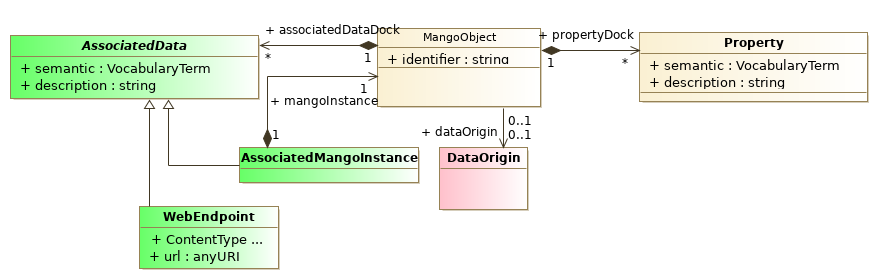
\includegraphics[width=1.0\textwidth]{../model/overview.png}
     \caption{Model overview}
     \label{overview}
\end{figure}

The root class of the model \texttt{MANGOObject} which has only
one mandatory attribute, an \texttt{identifier}.
Identifiers should be unique within a collection, e.g. a data table, although 
this feature is not required by the model.

In addition to its identifier, \texttt{MANGOObject} objects have 2 components:

\begin{itemize}[noitemsep,topsep=0pt,parsep=0pt,partopsep=0pt]

  \item \texttt{dataOrigin} (origin of the \texttt{MANGOObject}) : The structure of this class is based on
        the recommendations of the DCP interest group \footnote{https://ivoa.net/documents/DataOrigin/index.html}.
  \item \texttt{popertyDock} (place holder for all the \texttt{MANGOObject} properties) :
        This is an open-ended collection.
        Mango properties inherit from the base class \texttt{Property},
        which contains everything necessary to identify both their nature and their role.
        Properties can be linked together to form compound parameters.
\end{itemize}


\subsection{Properties}

      \begin{figure}[h]
        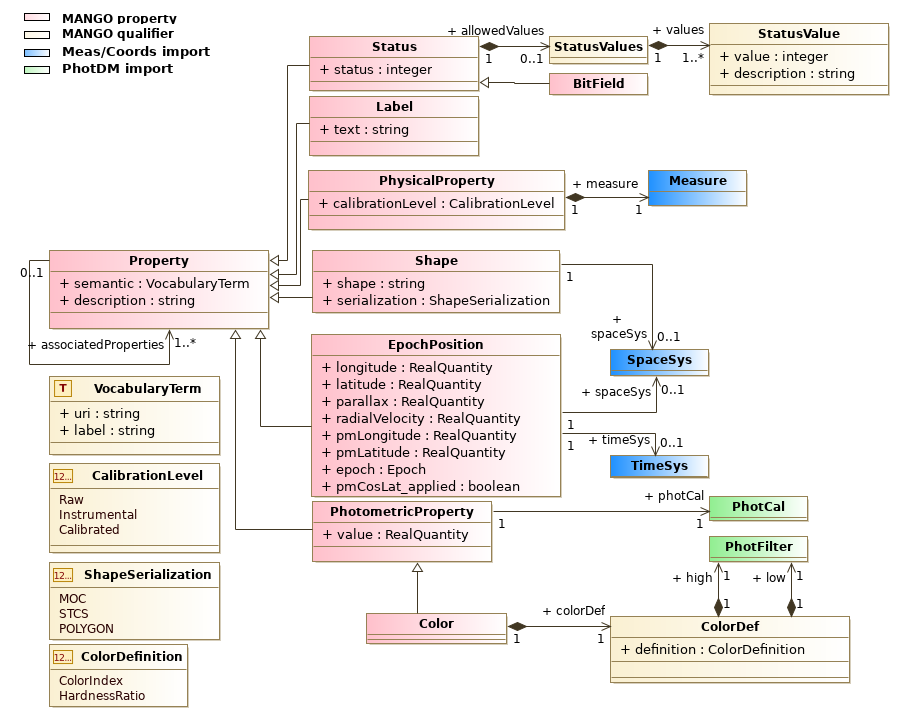
\includegraphics[width=1.0\textwidth]{../model/property.png}
        \caption{MANGO Properties}
        \label{fig:property}
      \end{figure}

\subsubsection{Property Identification}
Since the set of properties associated with a particular instance is not defined by the model,
MANGO cannot define a specific role for each property. However, the model provides different ways
for the client to understand the actual nature of each property:

\begin{itemize}[noitemsep,topsep=0pt,parsep=0pt,partopsep=0pt]
    \item \textbf{Class type}: often the scientific meaning of the quantity.
    \item \textbf{Semantics}: the semantic tag specifies the exact role of the property by
          referring to a standard vocabulary. The semantic tag can relate to the property itself
          or to the set formed by the property and its associated properties.
          For example, a signal amplitude associated with a time and position can be tagged
          as a photon event.
    \item \textbf{Description}: free text description.
    \item \textbf{Literal attributes} : some property classes embed qualifiers telling 
          how the quantity must be interpreted (e.g. colour vs hardness ratio)
\end{itemize}


\subsubsection{MANGO and MIVOT: Structuring Tabular Data}

MANGO is primarily used to organise tabular data provided by TAP services \citep{2019ivoa.spec.0927D}.
To achieve this, table rows must be linked to the model using MIVOT annotations.
We propose two strategies for establishing this mapping:
\begin{itemize}[noitemsep,topsep=0pt,parsep=0pt,partopsep=0pt]
    \item Single Object per Row: Each table row is treated as a single object,
          with its properties grouped within a container or dock.
    \item Scattered Independent Quantities: Each table row is considered as a collection of independent quantities.
\end{itemize}

MIVOT annotations support both approaches:

\begin{itemize}[noitemsep,topsep=0pt,parsep=0pt,partopsep=0pt]
    \item MANGO as a Global View: This configuration enables full utilisation of the 
          model's features. Properties can be interconnected, data rows can be identified
          and treated as individual entities (MANGO objects) that can be linked together to describe,
          for example, sources with their detections or orbiting systems.
          This approach allows for serialisation formats like XML or JSON, which often require
          a unique root.
          However, the annotation process might be slightly more complex due to additional class levels.
    \item MANGO as a Sparse Parameter View: In this simpler approach, the data mapping is a
          flat set of independent objects. Clients can iterate through these objects and process
          the entities of interest individually.
          It's important to note that such a client could also handle data mapped to the full MANGO schema.
          The annotation process might be less complex on the server side.
\end{itemize}

This document does not favour one approach over the other.
The decision ultimately rests with the data providers.
However, both options are based on the full-featured MANGO model.


% -------------------------------------------
% Items to substitute into the ivoatex document template.
%
%\ivoagroup{Data Model Working Group}

%\title{Mango}


%\author{Laurent Michel}
    
%\author{Fran??ois Bonnarel}
    
%\author{Gilles Landais}
    
%\author{Mireille Louys}
    
%\author{Marco Molinaro}
    
%\author{Jesue Salgado}
    
%\previousversion{0.0}
      
% -------------------------------------------

\pagebreak
\section{Model: mango }
  
  % INSERT FIGURE HERE
  %\begin{figure}[h]
  %\begin{center}
  %  \includegraphics[width=\textwidth]{????.png}
  %  \caption{???}\label{fig:????}
  %\end{center}
  %\end{figure}

  Data model based oon components and data association for source data

  \subsection{AssociatedMangoObject}
  \label{sect:AssociatedMangoObject}
    Class holder for linking the Mango object to another \texttt{MangoObject}.

    \subsubsection{AssociatedMangoObject.semantic}
      \textbf{vodml-id: AssociatedMangoObject.semantic} \newline
      \textbf{type: \hyperref[sect:VocabularyTerm]{mango:VocabularyTerm}} \newline
      \textbf{multiplicity: 1} \newline 
      Semantic concept giving the nature of the associated data.

    \subsubsection{AssociatedMangoObject.description}
      \textbf{vodml-id: AssociatedMangoObject.description} \newline
      \textbf{type: \hyperref[sect:ivoa]{ivoa:string}} \newline
      \textbf{multiplicity: 1} \newline 
      Free text description of the associated data

    \subsubsection{AssociatedMangoObject.mangoObject}
      \textbf{vodml-id: AssociatedMangoObject.mangoObject} \newline
      \textbf{type: \hyperref[sect:MangoObject]{mango:MangoObject}} \newline
      \textbf{multiplicity: 1} \newline 
      Reference of the associated \texttt{MangoObject}.

  \subsection{BitField}
  \label{sect:BitField}
    Property state for which each possible value is represented by a bit, so that multiple states can be contained in the same numerical value. The values defined in the related \texttt{StatusValues} must correspond to a bit patterns. This constraint is not enforced by the model.

  \subsection{Color}
  \label{sect:Color}
    Property that describes a color of the \texttt{MangoObject}. The color is not an intrinsic property of the MANGO object, but a value relative to two filters or energy bands.

    \subsubsection{Color.colorDef}
      \textbf{vodml-id: Color.colorDef} \newline
      \textbf{type: \hyperref[sect:ColorDef]{mango:ColorDef}} \newline
      \textbf{multiplicity: 1} \newline 
      Color definition. Can be either a difference of magnitudes or a hardness ratio.

  \subsection{ColorDef}
  \label{sect:ColorDef}
    Class holder for a color definition. This definition includes how the color is calculated (Mag or HR) and the filters on which the color is based. In case of hardness ratio, the energy bands must be modeled as instances of \texttt{photdm:PhotFilter} with a flat transfert function.

    \subsubsection{ColorDef.definition}
      \textbf{vodml-id: ColorDef.definition} \newline
      \textbf{type: \hyperref[sect:ColorDefinition]{mango:ColorDefinition}} \newline
      \textbf{multiplicity: 1} \newline 
      Attribute giving the way the color is calculated (Mag or HR).

    \subsubsection{ColorDef.high}
      \textbf{vodml-id: ColorDef.high} \newline
      \textbf{type: photdm:PhotFilter} \newline
      \textbf{multiplicity: 1} \newline 
      Reference to the \texttt{photdm:PhotFilter} corresponding the higher band of the color.

    \subsubsection{ColorDef.low}
      \textbf{vodml-id: ColorDef.low} \newline
      \textbf{type: photdm:PhotFilter} \newline
      \textbf{multiplicity: 1} \newline 
      Reference to the \texttt{photdm:PhotFilter} corresponding the lower band for that color.

  \subsection{EpochPosition}

      \begin{figure}[h]
        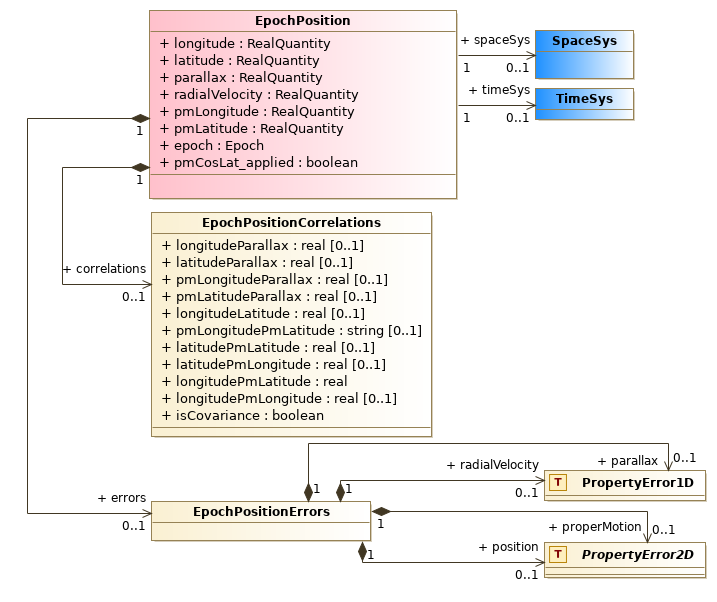
\includegraphics[width=1.0\textwidth]{../model/EpochPosition.png}
        \caption{Class EpochPosition}
        \label{fig:EpochPosition}
      \end{figure}

    
  \label{sect:EpochPosition}
    This class is a view of \texttt{Astronomical Coordinates and Coordinate Systems} components that have been put together to form a consistent description of the position of an object moving over time. It consists of a celestial position, a proper motion, a radial velocity and a parallax. All components share the same coordinate systems for both time and space coordinates. \begin{itemize} \item Both position and proper motion reuse the \texttt{coords:LonLatPoint} elements. \item The space coordinate system is imported from \texttt{coords:spaceSys}. \item The time coordinate system is imported from \texttt{coords:timeSys}. \end{itemize} The \texttt{EpochPosition} error is modeled by specific classes supporting covariance and/or correlation between components. All individual components have their own units which must be consistent to each others. This consistency is not enforced by the model.

    \subsubsection{EpochPosition.longitude}
      \textbf{vodml-id: EpochPosition.longitude} \newline
      \textbf{type: \hyperref[sect:ivoa]{ivoa:RealQuantity}} \newline
      \textbf{multiplicity: 1} \newline 
      The longitude of the Point, as a Quantity with angular units (see \texttt{coords:LonLatPoint.lon}.

    \subsubsection{EpochPosition.latitude}
      \textbf{vodml-id: EpochPosition.latitude} \newline
      \textbf{type: \hyperref[sect:ivoa]{ivoa:RealQuantity}} \newline
      \textbf{multiplicity: 1} \newline 
      The latitude of the Point, as a Quantity with angular units (see \texttt{coords:LonLatPoint.lat}.

    \subsubsection{EpochPosition.parallax}
      \textbf{vodml-id: EpochPosition.parallax} \newline
      \textbf{type: \hyperref[sect:ivoa]{ivoa:RealQuantity}} \newline
      \textbf{multiplicity: 1} \newline 
      The measured parallax in the coordinate system of the \texttt{EpochPosition} instance.

    \subsubsection{EpochPosition.radialVelocity}
      \textbf{vodml-id: EpochPosition.radialVelocity} \newline
      \textbf{type: \hyperref[sect:ivoa]{ivoa:RealQuantity}} \newline
      \textbf{multiplicity: 1} \newline 
      The measured Velocity along of the radius axis (see \texttt{meas:Velocity.coord}).

    \subsubsection{EpochPosition.pmLongitude}
      \textbf{vodml-id: EpochPosition.pmLongitude} \newline
      \textbf{type: \hyperref[sect:ivoa]{ivoa:RealQuantity}} \newline
      \textbf{multiplicity: 1} \newline 
      Velocity along the longitude axis in angular distance per unit time (see \texttt{meas:ProperMotion.coord}). The current version of the model only allows a representation in the Polar coordinate space.

    \subsubsection{EpochPosition.pmLatitude}
      \textbf{vodml-id: EpochPosition.pmLatitude} \newline
      \textbf{type: \hyperref[sect:ivoa]{ivoa:RealQuantity}} \newline
      \textbf{multiplicity: 1} \newline 
      Velocity along the latitude axis in angular distance per unit time (see \texttt{meas:ProperMotion.coord}). The current version of the model only allows a representation in the Polar coordinate space.

    \subsubsection{EpochPosition.epoch}
      \textbf{vodml-id: EpochPosition.epoch} \newline
      \textbf{type: coords:Epoch} \newline
      \textbf{multiplicity: 1} \newline 
      Position epoch expressed within the common time system (see \texttt{coords:epoch})

    \subsubsection{EpochPosition.pmCosLat\_applied}
      \textbf{vodml-id: EpochPosition.pmCosLat\_applied} \newline
      \textbf{type: \hyperref[sect:ivoa]{ivoa:boolean}} \newline
      \textbf{multiplicity: 1} \newline 
      It is common, though not universal, practice to quote longitudinal proper motion pre-multiplied by cos(latitude) so that the magnitude of the quantity is not affected by its longitudinal position. We do not constrain the value to one form or the other in this model. Instead, this flag enables providers to convey whether or not the factor has been applied (see \texttt{meas:ProperMotion.cosLat\_applied})

    \subsubsection{EpochPosition.errors}
      \textbf{vodml-id: EpochPosition.errors} \newline
      \textbf{type: \hyperref[sect:EpochPositionErrors]{mango:EpochPositionErrors}} \newline
      \textbf{multiplicity: 0..1} \newline 
      Reference to the combined errors of the \texttt{EpochPosition} components.

    \subsubsection{EpochPosition.correlations}
      \textbf{vodml-id: EpochPosition.correlations} \newline
      \textbf{type: \hyperref[sect:EpochPositionCorrelations]{mango:EpochPositionCorrelations}} \newline
      \textbf{multiplicity: 0..1} \newline 
      Reference to the correlations between the \texttt{EpochPosition} components.

    \subsubsection{EpochPosition.spaceSys}
      \textbf{vodml-id: EpochPosition.spaceSys} \newline
      \textbf{type: coords:SpaceSys} \newline
      \textbf{multiplicity: 0..1} \newline 
      System that applies the space coordinates.

    \subsubsection{EpochPosition.timeSys}
      \textbf{vodml-id: EpochPosition.timeSys} \newline
      \textbf{type: coords:TimeSys} \newline
      \textbf{multiplicity: 0..1} \newline 
      System that applies the time coordinates (the epoch).

  \subsection{EpochPositionCorrelations}
  \label{sect:EpochPositionCorrelations}
    Class holder for the correlation coefficients between the \texttt{EpochPosition} components.

    \subsubsection{EpochPositionCorrelations.longitudeParallax}
      \textbf{vodml-id: EpochPositionCorrelations.longitudeParallax} \newline
      \textbf{type: \hyperref[sect:ivoa]{ivoa:real}} \newline
      \textbf{multiplicity: 0..1} \newline 
      Correlation (or covariance) coefficient between the position longitude and the parallax

    \subsubsection{EpochPositionCorrelations.latitudeParallax}
      \textbf{vodml-id: EpochPositionCorrelations.latitudeParallax} \newline
      \textbf{type: \hyperref[sect:ivoa]{ivoa:real}} \newline
      \textbf{multiplicity: 0..1} \newline 
      Correlation (or covariance) coefficient between the position latitude and the parallax

    \subsubsection{EpochPositionCorrelations.pmLongitudeParallax}
      \textbf{vodml-id: EpochPositionCorrelations.pmLongitudeParallax} \newline
      \textbf{type: \hyperref[sect:ivoa]{ivoa:real}} \newline
      \textbf{multiplicity: 0..1} \newline 
      Correlation (or covariance) coefficient between the proper motion longitude and the parallax

    \subsubsection{EpochPositionCorrelations.pmLatitudeParallax}
      \textbf{vodml-id: EpochPositionCorrelations.pmLatitudeParallax} \newline
      \textbf{type: \hyperref[sect:ivoa]{ivoa:real}} \newline
      \textbf{multiplicity: 0..1} \newline 
      Correlation (or covariance) coefficient between the proper motion latitude and the parallax

    \subsubsection{EpochPositionCorrelations.longitudeLatitude}
      \textbf{vodml-id: EpochPositionCorrelations.longitudeLatitude} \newline
      \textbf{type: \hyperref[sect:ivoa]{ivoa:real}} \newline
      \textbf{multiplicity: 0..1} \newline 
      Correlation (or covariance) coefficient between the position longitude and the position latitude

    \subsubsection{EpochPositionCorrelations.pmLongitudePmLatitude}
      \textbf{vodml-id: EpochPositionCorrelations.pmLongitudePmLatitude} \newline
      \textbf{type: } \newline
      \textbf{multiplicity: 0..1} \newline 
      Correlation (or covariance) coefficient between the proper motion longitude and the proper motion latitude

    \subsubsection{EpochPositionCorrelations.latitudePmLatitude}
      \textbf{vodml-id: EpochPositionCorrelations.latitudePmLatitude} \newline
      \textbf{type: \hyperref[sect:ivoa]{ivoa:real}} \newline
      \textbf{multiplicity: 0..1} \newline 
      Correlation (or covariance) coefficient between the position latitude and the proper motion latitude

    \subsubsection{EpochPositionCorrelations.latitudePmLongitude}
      \textbf{vodml-id: EpochPositionCorrelations.latitudePmLongitude} \newline
      \textbf{type: \hyperref[sect:ivoa]{ivoa:real}} \newline
      \textbf{multiplicity: 0..1} \newline 
      Correlation (or covariance) coefficient between the position latitude and the proper motion longitude

    \subsubsection{EpochPositionCorrelations.longitudePmLatitude}
      \textbf{vodml-id: EpochPositionCorrelations.longitudePmLatitude} \newline
      \textbf{type: \hyperref[sect:ivoa]{ivoa:real}} \newline
      \textbf{multiplicity: 1} \newline 
      Correlation (or covariance) coefficient between the position longitude and the proper motion latitude

    \subsubsection{EpochPositionCorrelations.longitudePmLongitude}
      \textbf{vodml-id: EpochPositionCorrelations.longitudePmLongitude} \newline
      \textbf{type: \hyperref[sect:ivoa]{ivoa:real}} \newline
      \textbf{multiplicity: 0..1} \newline 
      Correlation (or covariance) coefficient between the position longitude and the proper motion longitude

    \subsubsection{EpochPositionCorrelations.isCovariance}
      \textbf{vodml-id: EpochPositionCorrelations.isCovariance} \newline
      \textbf{type: \hyperref[sect:ivoa]{ivoa:boolean}} \newline
      \textbf{multiplicity: 1} \newline 
      Boolean telling whether the correlations must be interpreted as covariance or as correlation coefficients.

  \subsection{EpochPositionErrors}
  \label{sect:EpochPositionErrors}
    Class holder for the errors of the EpochPosition attributes

    \subsubsection{EpochPositionErrors.parallax}
      \textbf{vodml-id: EpochPositionErrors.parallax} \newline
      \textbf{type: \hyperref[sect:error.PropertyError1D]{mango:error.PropertyError1D}} \newline
      \textbf{multiplicity: 0..1} \newline 
      Parallax error. This error is meant to be symmetrical

    \subsubsection{EpochPositionErrors.radialVelocity}
      \textbf{vodml-id: EpochPositionErrors.radialVelocity} \newline
      \textbf{type: \hyperref[sect:error.PropertyError1D]{mango:error.PropertyError1D}} \newline
      \textbf{multiplicity: 0..1} \newline 
      Error in the radial velocity. This error is meant to be symmetrical

    \subsubsection{EpochPositionErrors.position}
      \textbf{vodml-id: EpochPositionErrors.position} \newline
      \textbf{type: \hyperref[sect:error.PropertyError2D]{mango:error.PropertyError2D}} \newline
      \textbf{multiplicity: 0..1} \newline 
      Position error; can be an ellipse, a correlation matrix or a covariance matrix.

    \subsubsection{EpochPositionErrors.properMotion}
      \textbf{vodml-id: EpochPositionErrors.properMotion} \newline
      \textbf{type: \hyperref[sect:error.PropertyError2D]{mango:error.PropertyError2D}} \newline
      \textbf{multiplicity: 0..1} \newline 
      Position error; can be an ellipse, a correlation matrix or a covariance matrix.

  \subsection{Label}
  \label{sect:Label}
    Free text label seen as a MANGO object property.

    \subsubsection{Label.text}
      \textbf{vodml-id: Label.text} \newline
      \textbf{type: \hyperref[sect:ivoa]{ivoa:string}} \newline
      \textbf{multiplicity: 1} \newline 
      Text of label property of the MANGO object.

  \subsection{MangoObject}
  \label{sect:MangoObject}
    Central model class: applied to a data table, each row can be modelled as a MangoObject instance. Each MangoObject hosts a collection of physical or calculated parameters, a collection of associated data, a description of the data origin and an identifier.

    \subsubsection{MangoObject.identifier}
      \textbf{vodml-id: MangoObject.identifier} \newline
      \textbf{type: \hyperref[sect:ivoa]{ivoa:string}} \newline
      \textbf{multiplicity: 1} \newline 
      Unique identifier of the \texttt{MangoObject}. The uniqueness of that identifier is not managed by the model. The format is free.

    \subsubsection{MangoObject.propertyDock}
      \textbf{vodml-id: MangoObject.propertyDock} \newline
      \textbf{type: \hyperref[sect:Property]{mango:Property}} \newline
      \textbf{multiplicity: 0..*} \newline 
      Reference to the open-ended collection of the \texttt{MangoObject} properties (physical or calculated).

    \subsubsection{MangoObject.dataOrigin}
      \textbf{vodml-id: MangoObject.dataOrigin} \newline
      \textbf{type: \hyperref[sect:dataorigin.DataOrigin]{mango:dataorigin.DataOrigin}} \newline
      \textbf{multiplicity: 0..1} \newline 
      Reference to the description of the origin of the \texttt{MangoObject}.

    \subsubsection{MangoObject.associatedMangoObjects}
      \textbf{vodml-id: MangoObject.associatedMangoObjects} \newline
      \textbf{type: \hyperref[sect:AssociatedMangoObject]{mango:AssociatedMangoObject}} \newline
      \textbf{multiplicity: 0..*} \newline 
      Abstract reference to a particular dataset associated to the MANGO entity. This class is used to specify the type of the associated dataset as well as its role.

  \subsection{PhotometricProperty}
  \label{sect:PhotometricProperty}
    Observed brightness of the \texttt{MangoObject}. The distinction between fluxes and magnitudes is made by the unit. This property should refer to a photometric calibration as defined by the \texttt{PhotDM} model.

    \subsubsection{PhotometricProperty.value}
      \textbf{vodml-id: PhotometricProperty.value} \newline
      \textbf{type: \hyperref[sect:ivoa]{ivoa:RealQuantity}} \newline
      \textbf{multiplicity: 1} \newline 
      Value of the photometric property associated with a photometric calibration as defined by the \texttt{PhotDM} model.

    \subsubsection{PhotometricProperty.error}
      \textbf{vodml-id: PhotometricProperty.error} \newline
      \textbf{type: meas:Uncertainty} \newline
      \textbf{multiplicity: 0..1} \newline 
      Error on the \texttt{PhotometricProperty}, imported from \texttt{meas:Uncertainty}.

    \subsubsection{PhotometricProperty.photCal}
      \textbf{vodml-id: PhotometricProperty.photCal} \newline
      \textbf{type: photdm:PhotCal} \newline
      \textbf{multiplicity: 1} \newline 
      Photometric calibration that applies to the photometric property. It must be an instance of \texttt{photdm:PhotCal}.

  \subsection{PhysicalProperty}
  \label{sect:PhysicalProperty}
    Place holder for any quantity that can be hold by measure as defined in the \texttt{Astronomical Measurements Model}.

    \subsubsection{PhysicalProperty.calibrationLevel}
      \textbf{vodml-id: PhysicalProperty.calibrationLevel} \newline
      \textbf{type: \hyperref[sect:CalibrationLevel]{mango:CalibrationLevel}} \newline
      \textbf{multiplicity: 1} \newline 
      Calibration level of the property (ObsCore).

    \subsubsection{PhysicalProperty.measure}
      \textbf{vodml-id: PhysicalProperty.measure} \newline
      \textbf{type: meas:Measure} \newline
      \textbf{multiplicity: 1} \newline 
      Instance of \texttt{Astronomical Measurements Model} that holds the Property value(s).

  \subsection{Property}
  \label{sect:Property}
    Class holder for a particular property, either physical or calculated, of the MANGO object. This class specifies both type and role of the property, and hosts the property instance itself.

    \noindent \textbf{constraint} \newline
    \indent    \textbf{detail: Property.One association at the time
 }\newline


    \subsubsection{Property.semantics}
      \textbf{vodml-id: Property.semantics} \newline
      \textbf{type: \hyperref[sect:VocabularyTerm]{mango:VocabularyTerm}} \newline
      \textbf{multiplicity: 1} \newline 
      Reference to a semantic concept giving the nature of the property or of the set made of the property and its associated properties.

    \subsubsection{Property.description}
      \textbf{vodml-id: Property.description} \newline
      \textbf{type: \hyperref[sect:ivoa]{ivoa:string}} \newline
      \textbf{multiplicity: 1} \newline 
      Free text description of the property or of the set made of the property and its associated properties.

    \subsubsection{Property.associatedProperties}
      \textbf{vodml-id: Property.associatedProperties} \newline
      \textbf{type: \hyperref[sect:Property]{mango:Property}} \newline
      \textbf{multiplicity: 1..*} \newline 
      Open-ended collection of MANGO properties associated with the \texttt{MangoObject}. These relationships are typically used to associate physical properties with time stamps and/or quality factors.

  \subsection{Shape}
  \label{sect:Shape}
    Description of the spatial extension of the MANGO object (for e.g. dust clouds).

    \subsubsection{Shape.shape}
      \textbf{vodml-id: Shape.shape} \newline
      \textbf{type: \hyperref[sect:ivoa]{ivoa:string}} \newline
      \textbf{multiplicity: 1} \newline 
      String serialization of the spatial extension of the \texttt{MangoObject}.

    \subsubsection{Shape.serialization}
      \textbf{vodml-id: Shape.serialization} \newline
      \textbf{type: \hyperref[sect:ShapeSerialization]{mango:ShapeSerialization}} \newline
      \textbf{multiplicity: 1} \newline 
      Serialization mode of the spatial extension of the MANGO entity.

    \subsubsection{Shape.spaceSys}
      \textbf{vodml-id: Shape.spaceSys} \newline
      \textbf{type: coords:SpaceSys} \newline
      \textbf{multiplicity: 0..1} \newline 
      Coordinate system that applies for the shape.

  \subsection{Status}
  \label{sect:Status}
    Property representing a status defined by a integer number that can only take on a defined number of values, each with its own description. Boolean status can be represented by \texttt{StatusValues} with 2 values e.g. 0 for False and 1 for True.

    \subsubsection{Status.status}
      \textbf{vodml-id: Status.status} \newline
      \textbf{type: \hyperref[sect:ivoa]{ivoa:integer}} \newline
      \textbf{multiplicity: 1} \newline 
      Actual value of the status.

    \subsubsection{Status.allowedValues}
      \textbf{vodml-id: Status.allowedValues} \newline
      \textbf{type: \hyperref[sect:StatusValues]{mango:StatusValues}} \newline
      \textbf{multiplicity: 0..1} \newline 
      List of the allowed values for the status. Each value has its own free text description.

  \subsection{StatusValue}
  \label{sect:StatusValue}
    Value allowed for a status, contain the value with a free text description.

    \subsubsection{StatusValue.value}
      \textbf{vodml-id: StatusValue.value} \newline
      \textbf{type: \hyperref[sect:ivoa]{ivoa:integer}} \newline
      \textbf{multiplicity: 1} \newline 
      Allowed value for a \texttt{Status}

    \subsubsection{StatusValue.description}
      \textbf{vodml-id: StatusValue.description} \newline
      \textbf{type: \hyperref[sect:ivoa]{ivoa:string}} \newline
      \textbf{multiplicity: 1} \newline 
      Free text description on the allowed value for a \texttt{Status}

  \subsection{StatusValues}
  \label{sect:StatusValues}
    Class holder for the list of the allowed values for the status.

    \subsubsection{StatusValues.values}
      \textbf{vodml-id: StatusValues.values} \newline
      \textbf{type: \hyperref[sect:StatusValue]{mango:StatusValue}} \newline
      \textbf{multiplicity: 1..*} \newline 
      List of the allowed values for the status. Each value has its own textual description.

  \subsection{VocabularyTerm}
  \label{sect:VocabularyTerm}
    Class holder for a term of a standardized vocabulary that applies to a property.

    \subsubsection{VocabularyTerm.uri}
      \textbf{vodml-id: VocabularyTerm.uri} \newline
      \textbf{type: \hyperref[sect:ivoa]{ivoa:string}} \newline
      \textbf{multiplicity: 1} \newline 
      URI the vocabulary term.

    \subsubsection{VocabularyTerm.label}
      \textbf{vodml-id: VocabularyTerm.label} \newline
      \textbf{type: \hyperref[sect:ivoa]{ivoa:string}} \newline
      \textbf{multiplicity: 1} \newline 
      Label attached to the vocabulary term. This is necessary because the URI may not contain any explicit label. This was the case for the IUA vocabulary until the Registry WG introduced rewriting rules that fix the issue.

  \subsection{WebEndpoint}
  \label{sect:WebEndpoint}
    Associated data referenced by an URL.

    \subsubsection{WebEndpoint.content\_type}
      \textbf{vodml-id: WebEndpoint.content\_type} \newline
      \textbf{type: \hyperref[sect:ivoa]{ivoa:string}} \newline
      \textbf{multiplicity: 1} \newline 
      URL mime type.

    \subsubsection{WebEndpoint.access\_url}
      \textbf{vodml-id: WebEndpoint.access\_url} \newline
      \textbf{type: \hyperref[sect:ivoa]{ivoa:anyURI}} \newline
      \textbf{multiplicity: 1} \newline 
      Web end-point.

    \subsubsection{WebEndpoint.content\_qualifier}
      \textbf{vodml-id: WebEndpoint.content\_qualifier} \newline
      \textbf{type: \hyperref[sect:ivoa]{ivoa:string}} \newline
      \textbf{multiplicity: 1} \newline 
      TODO : Missing description : please, update your UML model asap.

    \subsubsection{WebEndpoint.local\_semantics}
      \textbf{vodml-id: WebEndpoint.local\_semantics} \newline
      \textbf{type: \hyperref[sect:ivoa]{ivoa:string}} \newline
      \textbf{multiplicity: 1} \newline 
      TODO : Missing description : please, update your UML model asap.

  \subsection{ShapeFrame}
  \label{sect:ShapeFrame}

  Possible schemes to encode a shape in a string

  \noindent \underline{Enumeration Literals}
  \vspace{-\parsep}
  \small
  \begin{itemize}
  
    \item[\textbf{STC\_S}]: \textbf{vodml-id:} ShapeFrame.STC\_S \newline
          \textbf{description:} MOC serialization
    \item[\textbf{MOC}]: \textbf{vodml-id:} ShapeFrame.MOC \newline
          \textbf{description:} STCs serialization
  \end{itemize}
  \normalsize


  \subsection{ShapeSerialization}
  \label{sect:ShapeSerialization}

  Enumeration of the supported serialization modes for the shapes

  \noindent \underline{Enumeration Literals}
  \vspace{-\parsep}
  \small
  \begin{itemize}
  
    \item[\textbf{MOC}]: \textbf{vodml-id:} ShapeSerialization.MOC \newline
          \textbf{description:} Label indicating that the shape has been serialized as a S-MOC
    \item[\textbf{STCS}]: \textbf{vodml-id:} ShapeSerialization.STCS \newline
          \textbf{description:} Label indicating that the shape has been serialized as a STCS string
    \item[\textbf{POLYGON}]: \textbf{vodml-id:} ShapeSerialization.POLYGON \newline
          \textbf{description:} Label indicating that the shape has been serialized as a polygon (cf xtypes)
  \end{itemize}
  \normalsize


  \subsection{CalibrationLevel}
  \label{sect:CalibrationLevel}

  Enumeration of different possible calibration status of the property (Obscore)

  \noindent \underline{Enumeration Literals}
  \vspace{-\parsep}
  \small
  \begin{itemize}
  
    \item[\textbf{Raw}]: \textbf{vodml-id:} CalibrationLevel.Raw \newline
          \textbf{description:} Raw instrumental data, in a proprietary or internal data provider defined format, that needs instrument specific tools to be handled (ObsCore)
    \item[\textbf{Instrumental}]: \textbf{vodml-id:} CalibrationLevel.Instrumental \newline
          \textbf{description:} Instrumental data in a standard format which could be manipulated with standard astronomical packages (ObsCore).
    \item[\textbf{Calibrated}]: \textbf{vodml-id:} CalibrationLevel.Calibrated \newline
          \textbf{description:} Science ready data with the instrument signature removed (ObsCore)
  \end{itemize}
  \normalsize


  \subsection{ColorDefinition}
  \label{sect:ColorDefinition}

  Enumeration of the different types of colors supported by the model.

  \noindent \underline{Enumeration Literals}
  \vspace{-\parsep}
  \small
  \begin{itemize}
  
    \item[\textbf{ColorIndex}]: \textbf{vodml-id:} ColorDefinition.ColorIndex \newline
          \textbf{description:} Difference of magnitudes: typically $M_B - M_v$
    \item[\textbf{HardnessRatio}]: \textbf{vodml-id:} ColorDefinition.HardnessRatio \newline
          \textbf{description:} Normalized ratio of fluxes: $(F_{EB2} - F_{EB1}) / (F_{EB2} + F_{EB1})$
  \end{itemize}
  \normalsize


\pagebreak
\section{Package: error }
  \begin{figure}[h]
    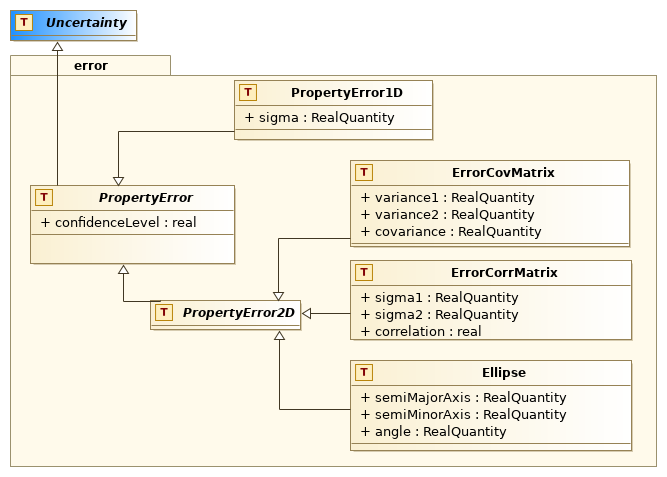
\includegraphics[width=1.0\textwidth]{../model/error.png}
    \caption{package error}
    \label{fig:error}
  \end{figure}



  % INSERT FIGURE HERE
  %\begin{figure}[h]
  %\begin{center}
  %  \includegraphics[width=\textwidth]{????.png}
  %  \caption{???}\label{fig:????}
  %\end{center}
  %\end{figure}

  The \texttt{error} package groups the MANGO built-in error classes. All these classes are derived from \texttt{meas:Uncertainty} to make them reusable by \texttt{meas:Measure} instances. Mango errors all have an attribute that specifies the confidence level

  \subsection{Ellipse}
  \label{sect:error.Ellipse}
    Elliptic error for 2D parameters such as sky positions. Major axis and minor axis have their own units, which must be the same for both. This is not enforced by the model.

    \subsubsection{Ellipse.semiMajorAxis}
      \textbf{vodml-id: error.Ellipse.semiMajorAxis} \newline
      \textbf{type: \hyperref[sect:ivoa]{ivoa:RealQuantity}} \newline
      \textbf{multiplicity: 1} \newline 
      Half of the ellipse major axis

    \subsubsection{Ellipse.semiMinorAxis}
      \textbf{vodml-id: error.Ellipse.semiMinorAxis} \newline
      \textbf{type: \hyperref[sect:ivoa]{ivoa:RealQuantity}} \newline
      \textbf{multiplicity: 1} \newline 
      Half of the ellipse minor axis

    \subsubsection{Ellipse.angle}
      \textbf{vodml-id: error.Ellipse.angle} \newline
      \textbf{type: \hyperref[sect:ivoa]{ivoa:RealQuantity}} \newline
      \textbf{multiplicity: 1} \newline 
      Angle between the North Polar Cape (NCP) and the major axis. This angle must be positive taking into account that angles are positive from North to the East. The angle has its own unit.

  \subsection{ErrorCorrMatrix}
  \label{sect:error.ErrorCorrMatrix}
    Correlation matrix for the error of a 2D quantities. The correlation matrix is symmetrical.

    \subsubsection{ErrorCorrMatrix.sigma1}
      \textbf{vodml-id: error.ErrorCorrMatrix.sigma1} \newline
      \textbf{type: \hyperref[sect:ivoa]{ivoa:RealQuantity}} \newline
      \textbf{multiplicity: 1} \newline 
      Error on the first dimension (right ascension in case of sky coordinates)

    \subsubsection{ErrorCorrMatrix.sigma2}
      \textbf{vodml-id: error.ErrorCorrMatrix.sigma2} \newline
      \textbf{type: \hyperref[sect:ivoa]{ivoa:RealQuantity}} \newline
      \textbf{multiplicity: 1} \newline 
      Error on the second dimension (declination in case of sky coordinates)

    \subsubsection{ErrorCorrMatrix.correlation}
      \textbf{vodml-id: error.ErrorCorrMatrix.correlation} \newline
      \textbf{type: \hyperref[sect:ivoa]{ivoa:real}} \newline
      \textbf{multiplicity: 1} \newline 
      Correlation coefficient between the 2 axis

  \subsection{ErrorCovMatrix}
  \label{sect:error.ErrorCovMatrix}
    Covariance matrix for the error of a 2D quantities. The covariance matrix is symmetrical.

    \subsubsection{ErrorCovMatrix.variance1}
      \textbf{vodml-id: error.ErrorCovMatrix.variance1} \newline
      \textbf{type: \hyperref[sect:ivoa]{ivoa:RealQuantity}} \newline
      \textbf{multiplicity: 1} \newline 
      Variance of the first dimension (right ascension in case of sky coordinates)

    \subsubsection{ErrorCovMatrix.variance2}
      \textbf{vodml-id: error.ErrorCovMatrix.variance2} \newline
      \textbf{type: \hyperref[sect:ivoa]{ivoa:RealQuantity}} \newline
      \textbf{multiplicity: 1} \newline 
      Variance of the second dimension (declination in case of sky coordinates)

    \subsubsection{ErrorCovMatrix.covariance}
      \textbf{vodml-id: error.ErrorCovMatrix.covariance} \newline
      \textbf{type: \hyperref[sect:ivoa]{ivoa:RealQuantity}} \newline
      \textbf{multiplicity: 1} \newline 
      Covariance of the 2 axis

  \subsection{PropertyError (Abstract)}
  \label{sect:error.PropertyError}
    Root (abstract) class of the errors that can be attached to a MANGO property. The class inherits from \texttt{meas:uncertainty} in order to be usable in the context of properties based on \texttt{Measures} classes.

    \subsubsection{PropertyError.confidenceLevel}
      \textbf{vodml-id: error.PropertyError.confidenceLevel} \newline
      \textbf{type: \hyperref[sect:ivoa]{ivoa:real}} \newline
      \textbf{multiplicity: 1} \newline 
      Confidence level of the error. The confidence level must be in $[0, 1]$ (not enforced by the VO-DML schema).

  \subsection{PropertyError1D}
  \label{sect:error.PropertyError1D}
    Symetrical error for 1D parameters

    \subsubsection{PropertyError1D.sigma}
      \textbf{vodml-id: error.PropertyError1D.sigma} \newline
      \textbf{type: \hyperref[sect:ivoa]{ivoa:RealQuantity}} \newline
      \textbf{multiplicity: 1} \newline 
      Magnitude of error on a one-dimensional parameter

  \subsection{PropertyError2D (Abstract)}
  \label{sect:error.PropertyError2D}
    Super (abstract) class for all errors of 2D parameters

\pagebreak
\section{Package: dataorigin }
  \begin{figure}[h]
    \includegraphics[width=1.0\textwidth]{../model/dataorigin.png}
    \caption{package dataorigin}
    \label{fig:dataorigin}
  \end{figure}



  % INSERT FIGURE HERE
  %\begin{figure}[h]
  %\begin{center}
  %  \includegraphics[width=\textwidth]{????.png}
  %  \caption{???}\label{fig:????}
  %\end{center}
  %\end{figure}

  Package grouping together all the components needed to model the origin of \texttt{MangoObject}.

  \subsection{Article}
  \label{sect:dataorigin.Article}
    Reference article for the MANGO entity

    \subsubsection{Article.editor}
      \textbf{vodml-id: dataorigin.Article.editor} \newline
      \textbf{type: \hyperref[sect:ivoa]{ivoa:string}} \newline
      \textbf{multiplicity: 1} \newline 
      Editor name (article)

    \subsubsection{Article.article}
      \textbf{vodml-id: dataorigin.Article.article} \newline
      \textbf{type: \hyperref[sect:ivoa]{ivoa:string}} \newline
      \textbf{multiplicity: 1} \newline 
      Bibcode or DOI of the reference article

  \subsection{DataOrigin}
  \label{sect:dataorigin.DataOrigin}
    Class representing the origin of the data following the DCP note (TBD)

    \subsubsection{DataOrigin.citation}
      \textbf{vodml-id: dataorigin.DataOrigin.citation} \newline
      \textbf{type: \hyperref[sect:ivoa]{ivoa:string}} \newline
      \textbf{multiplicity: 1} \newline 
      Dataset identifier that can be used for citation (e.g. DOI)

    \subsubsection{DataOrigin.reference\_url}
      \textbf{vodml-id: dataorigin.DataOrigin.reference\_url} \newline
      \textbf{type: \hyperref[sect:ivoa]{ivoa:string}} \newline
      \textbf{multiplicity: 1} \newline 
      Dataset landing page

    \subsubsection{DataOrigin.resource\_version}
      \textbf{vodml-id: dataorigin.DataOrigin.resource\_version} \newline
      \textbf{type: \hyperref[sect:ivoa]{ivoa:string}} \newline
      \textbf{multiplicity: 1} \newline 
      Dataset version

    \subsubsection{DataOrigin.creator}
      \textbf{vodml-id: dataorigin.DataOrigin.creator} \newline
      \textbf{type: \hyperref[sect:ivoa]{ivoa:string}} \newline
      \textbf{multiplicity: 1} \newline 
      Person(s) mainly involved in the creation of the resource, generally the author

    \subsubsection{DataOrigin.cites}
      \textbf{vodml-id: dataorigin.DataOrigin.cites} \newline
      \textbf{type: \hyperref[sect:ivoa]{ivoa:string}} \newline
      \textbf{multiplicity: 1} \newline 
      Identifier (IVOID, DOI or Bibcode) of a second Resource using relation of type \texttt{cites} (\url{https://www.ivoa.net/rdf/voresource/relationship\_type/})

    \subsubsection{DataOrigin.is\_derived\_from}
      \textbf{vodml-id: dataorigin.DataOrigin.is\_derived\_from} \newline
      \textbf{type: \hyperref[sect:ivoa]{ivoa:string}} \newline
      \textbf{multiplicity: 1} \newline 
      Identifier (IVOID, DOI or Bibcode) of a second resource using relation of type \texttt{is\_derived\_from} (\url{https://www.ivoa.net/rdf/voresource/relationship\_type/})

    \subsubsection{DataOrigin.original\_date}
      \textbf{vodml-id: dataorigin.DataOrigin.original\_date} \newline
      \textbf{type: \hyperref[sect:ivoa]{ivoa:datetime}} \newline
      \textbf{multiplicity: 1} \newline 
      Date of the original resource from which the MANGO object is derived

    \subsubsection{DataOrigin.query}
      \textbf{vodml-id: dataorigin.DataOrigin.query} \newline
      \textbf{type: \hyperref[sect:dataorigin.QueryOrigin]{mango:dataorigin.QueryOrigin}} \newline
      \textbf{multiplicity: 0..1} \newline 
      Description of the request from which the data originates.

    \subsubsection{DataOrigin.rights}
      \textbf{vodml-id: dataorigin.DataOrigin.rights} \newline
      \textbf{type: \hyperref[sect:dataorigin.License]{mango:dataorigin.License}} \newline
      \textbf{multiplicity: 0..1} \newline 
      Reference to the rights that apply to the data.

    \subsubsection{DataOrigin.article}
      \textbf{vodml-id: dataorigin.DataOrigin.article} \newline
      \textbf{type: \hyperref[sect:dataorigin.Article]{mango:dataorigin.Article}} \newline
      \textbf{multiplicity: 0..1} \newline 
      Reference to the article from which the data originates.

  \subsection{License}
  \label{sect:dataorigin.License}
    Place holder for the license covering the MANGO instance

    \subsubsection{License.rights\_uri}
      \textbf{vodml-id: dataorigin.License.rights\_uri} \newline
      \textbf{type: \hyperref[sect:ivoa]{ivoa:string}} \newline
      \textbf{multiplicity: 1} \newline 
      Licence URI. Following Registry practice, this should come from SPDX https://spdx.org/licenses/, though Creative Commons URLs https://creativecommons.org are also admitted.

    \subsubsection{License.rights}
      \textbf{vodml-id: dataorigin.License.rights} \newline
      \textbf{type: \hyperref[sect:ivoa]{ivoa:string}} \newline
      \textbf{multiplicity: 1} \newline 
      License or Copyright text

  \subsection{QueryOrigin}
  \label{sect:dataorigin.QueryOrigin}
    Description of the query the MANGO instance results from.

    \subsubsection{QueryOrigin.ivoid}
      \textbf{vodml-id: dataorigin.QueryOrigin.ivoid} \newline
      \textbf{type: \hyperref[sect:ivoa]{ivoa:string}} \newline
      \textbf{multiplicity: 1} \newline 
      IVOID of the underlying data collection

    \subsubsection{QueryOrigin.publisher}
      \textbf{vodml-id: dataorigin.QueryOrigin.publisher} \newline
      \textbf{type: \hyperref[sect:ivoa]{ivoa:string}} \newline
      \textbf{multiplicity: 1} \newline 
      Data center that produced the MANGO instance

    \subsubsection{QueryOrigin.server\_software}
      \textbf{vodml-id: dataorigin.QueryOrigin.server\_software} \newline
      \textbf{type: \hyperref[sect:ivoa]{ivoa:string}} \newline
      \textbf{multiplicity: 1} \newline 
      Version of the software the produced the MANGO object instance. It is encouraged to follow \url{https://ivoa.net/documents/Notes/softid/index.html}.

    \subsubsection{QueryOrigin.service\_protocol}
      \textbf{vodml-id: dataorigin.QueryOrigin.service\_protocol} \newline
      \textbf{type: \hyperref[sect:ivoa]{ivoa:string}} \newline
      \textbf{multiplicity: 1} \newline 
      IVOID of the protocol through which the data was retrieved

    \subsubsection{QueryOrigin.request}
      \textbf{vodml-id: dataorigin.QueryOrigin.request} \newline
      \textbf{type: \hyperref[sect:ivoa]{ivoa:string}} \newline
      \textbf{multiplicity: 1} \newline 
      Full request URL including a query string. For the simple protocols,put the url-encoded form of the query parameters. For TAP queries, use the /sync UWS URL. The format is free for others request types.

    \subsubsection{QueryOrigin.query}
      \textbf{vodml-id: dataorigin.QueryOrigin.query} \newline
      \textbf{type: \hyperref[sect:ivoa]{ivoa:string}} \newline
      \textbf{multiplicity: 1} \newline 
      Input query in a formal langage such as ADQL.equest types

    \subsubsection{QueryOrigin.request\_date}
      \textbf{vodml-id: dataorigin.QueryOrigin.request\_date} \newline
      \textbf{type: \hyperref[sect:ivoa]{ivoa:datetime}} \newline
      \textbf{multiplicity: 1} \newline 
      Query execution date

    \subsubsection{QueryOrigin.contact}
      \textbf{vodml-id: dataorigin.QueryOrigin.contact} \newline
      \textbf{type: \hyperref[sect:ivoa]{ivoa:string}} \newline
      \textbf{multiplicity: 1} \newline 
      Email or URL to contact the publisher


\section{Integrating MANGO with TAP Services}

This non-normative section describes potential strategies for
storing and discovering MANGO instances within TAP services.
We assume that the TAP service hosts catalogs containing MANGO instances,
referred to as  \emph{MANGO Catalogs}.

\subsection{Storing MANGO Catalogs in TAP}
For now, we'll focus on storing the properties of MANGO instances. 

The tabular structure of MANGO instances will be reflected in TAP services as three tables:

\begin{itemize}
  \item One single master table for catalogs, including various metadata beyond the scope of
        MANGO and a unique identifier (primary key).
  \item One master sources table for source instances, containing the catalog identifier
        and a primary key that is more robust than the MANGO identifier.
  \item Individual tables for each supported parameter, with a foreign key
        linking to the master sources table.
\end{itemize}

While the measure model is hierarchical, it can be flattened into a single table,
considering that the model structure can be retrieved using TAP\_SCHEMA.
This schema necessitates server-side exploration of all parameter tables
to retrieve complete MANGO instances.
To speed-up this process, the \emph{MANGOCore} table can be utilised.

\subsection{ \emph{MANGOCore} Table}

The discovery of \emph{MANGO Catalogs} can be helped by a  \emph{MANGOCore} table located in the  \emph{schema} schema. As MANGO is not dedicated to any specific domain, we cannot define a set of core parameters, but parameters can be flagged as \emph{Core Parameter}.
This selection is left at the discretion of the curator.
The \emph{MANGOCore} table has set of columns per parameter class plus one for the catalog ID.
It has one row per stored catalog. Each parameter has at least 2 columns: one with the UCD and one with the \emph{Core} flag. TBC


\appendix

% \section{Gaia}
% Gaia mission is producing the largest and more precise 3D map of our galaxy.

Gaia core solution is able to solve the astrometric solution of more than 1
billion sources by complex models and algorithms \citep{2012A&A...538A..78L}.
Using a minimisation problem approach, different detections identified on
different scans can be associated to the same astronomical source. Some of the
properties would be direct measurements on single scans (e.g. positions or
magnitudes). Also other properties like radial velocity (measured in redshift
units) are also obtained at integration time of the scans.

Once detections on different scans are associated to a single astronomical
source, these direct measurements can be combined to generate derived
measurements. Trajectories on the sky for galactic objects are seen as
spirals including the combination of the proper motion of the object
(derived by the main vector of movement of the source) and the parallax
(derived by the radius of the apparent spiral produced by the different
angles of the Gaia observations at different periods).

From these properties, others could be also derived like, e.g. the distance,
although the exact transformation from parallax to distance requires the use of
accurate calculations and calibrations so, in general, only direct astrometric
properties, like parallax, are usually provided into the catalogues.

Finally, other properties will be also obtained by the cross-identification of
detections as a single astronomical source. For example, time series could be
combined as the result of measurements of magnitudes from different scans
detections.

Although it is not its main scientific target and apart from stellar objects,
other extra-galactic sources could be also studied with Gaia. For example, QSOs
are observed by Gaia as point-like sources with zero proper motion. For these
kind of sources, typical extra-galactic properties like, redshift, could be also
provided.

A non-exhaustive list of properties required for Gaia use cases would be composed
of:

\begin{itemize}
    \item identifier
    \item sky reference position
    \item proper motion
    \item parallax and distance

    \item source extension
    \item radial velocity
    \item redshift
    \item photometry
    \item date of detection
    \item correlation
    \item multiple detection
\end{itemize}

% \section{Euclid}
% Euclid telescope has been designed to unveil some of the questions about the
dark Universe, including dark matter and dark energy, what would include, e.g.
quite accurate measurements of the expansion of the Universe.

Euclid will mainly observe extragalactic objects providing, e.g. information
of the shapes of galaxies, gravitational lensing,  baryon acoustic oscillations
and distances to galaxies using spectroscopic data.

For this mission, and apart from the common metadata provided for extra galactic
sources into astronomical catalogues, a good support for object taxonomy and
shapes of objects will be required. As known due to general relativity effects,
shapes far galaxies could be deformed due to gravitational lensing effects,
producing convergence (visual displacements on the position) and rear (deformation
of the shape) effects. All these metadata should be ready for annotations and,
also, correlated to theoretical or real metadata in other datasets.

Finally, crossmatch information with other catalogues will be of crucial interest
as data from other satellites and, more importantly, from ground based
observatories will be combined with Euclid data to produce consistent scientific
datasets.

A non-exhaustive list of properties required for Euclid use cases would be composed
of:
\begin{itemize}
    \item identifier
    \item sky position
    \item correlation with other catalogues
    \item photometry (ground + satellite )
    \item morphology class
    \item redshift
    \item photometric redshift
\end{itemize}

\section{Chandra Archive}
\label{sec:chandra} 
The Chandra Source Catalog(CSC) is the definitive catalog of serendipitous X-ray sources identified in
publicly released imaging observations obtained by NASA’s ChandraX-ray Observatory (CXO).  The CSC is
developed and published by the ChandraX-ray Center (CXC) and is supported by NASA contract NAS 8-3060
to the Smithsonian Astrophysical Observatory for operation of the CXC.  CSC Release 2.0 (Oct. 2019) includes
properties for approximately 316,000 X-ray sources on the sky extracted from about 375,000 detections.
%\TODO{ cite\{chandra\_whitepaper, 2019\} }

The catalog itself consists of approximately 1,700 columns covering properites at the individual observation and stacked analysis levels.
Table \ref{tab:chandra_props} summarizes some of the basic catalog properties derived from standard CSCView queries.
%However, properties that fully characterize variability, as well as spectral and photometric properties are also included in the catalog.

\begin{table}[ht!]
  \tiny
  \begin{tabular}{|p{0.4cm}p{10.0cm}|}
    \hline
    \multicolumn{2}{|l|}{\textbf{Per Source:}} \\
    & \texttt{ Source name } \\
    & \texttt{ Source position and position errors } \\
    & \texttt{ Significance of the source (signal to noise) } \\
    & \texttt{ Likelihood of the source  (True, False, or Marginal detection) } \\
    & \texttt{ Source extent flag } \\
    & \texttt{ Variability flag } \\
    & \texttt{ Spectral variability flag } \\
    & \texttt{ Fluxes and flux errors in ACIS bands b, h, m, s, u } \\
    & \texttt{ Flux and flux error in  HRC band w } \\
    & \texttt{ Hardness ratios and errors for hm, hs, ms colors } \\
    & \texttt{ Short term (intra-obs) variability probability for each band } \\
    & \texttt{ Long term (inter-obs) variability probability for each band } \\
    & \texttt{ Spectral (hardness ratios) variability for each color } \\
    \hline
    \multicolumn{2}{|l|}{\textbf{Per Detection (at the stack level):}} \\
    & \texttt{ Detection ID } \\
    & \texttt{ Detection position and position errors } \\
    & \texttt{ Flux significance of the detection (S/N) } \\
    & \texttt{ Detection likelihood (True, False, or marginal detection?) } \\
    & \texttt{ Source extent code (codification of source extent in different bands) } \\
    & \texttt{ Variability flag } \\
    & \texttt{ Spectral variability flag } \\
    & \texttt{ Fluxes and flux errors in ACIS bands b, h, m, s, u } \\
    & \texttt{ Flux and flux error in  HRC band w } \\
    & \texttt{ Hardness ratios and errors for hm, hs, ms colors } \\
    & \texttt{ Short term (intra-obs) variability probability for each band } \\
    & \texttt{ Long term (inter-obs) variability probability for each band } \\
    & \texttt{ Spectral (hardness ratios) variability probability for each color } \\
    \hline
    \multicolumn{2}{|l|}{\textbf{Per Detection (at the observation level):}} \\
    \multicolumn{2}{|l|}{ Note that source detection is done at the stack level, but properties are estimated for the } \\
    \multicolumn{2}{|l|}{detections at each observation using the detection region from the stack level.} \\
    & \texttt{ Detection ID } \\
    & \texttt{ Detection position and position errors } \\
    & \texttt{ Flux significance of the detection (S/N) } \\
    & \texttt{ Detection likelihood } \\
    & \texttt{ Source extent code (codification of source extent in different bands) } \\
    & \texttt{ Variability code (applies to intra-obs only) } \\
    & \texttt{ Fluxes and flux errors in ACIS bands b, h, m, s, u } \\
    & \texttt{ Flux and flux error in  HRC band w } \\
    & \texttt{ Hardness ratios and errors for hm, hs, ms colors } \\
    & \texttt{ Short term (intra-obs) variability probability for each band } \\
    \hline

  \end{tabular}
  \caption{ Example Chandra Source Catalog Properties }
  \label{tab:chandra_props}

 \end{table}

The following are some example usage threads which can be facilitated by this model.
We provide a high-level summary here described in generic terms.  For each case, we
are generating detailed threads describing how each would be implemented using the
Chandra Source Catalog.

Note: Most of these cases have been simplified to a level appropriate for this version
of the model.  More complete and accurate science threads could be defined using more
complex types and associations which are out of the the current scope.

\begin{enumerate}
\item  Searching for spectrally variable or flaring point sources:
  \begin{itemize}
  \item Identifying spectrally variable point sources
    \begin{enumerate}
    \item From a catalog, identify a set of point sources with multiple spectrally-resolved observations
      \begin{itemize}
        \item Sources are classified as point sources or have a source extent that is consistent with being a point source
        \item Observations include detection properties in at least two user-specified wavebands
        \item There are multiple observations associated with the source
        \item If the catalog differentiates between detections and sources, each included detection must be uniquely associated with the source
      \end{itemize}
    \item From the set identified in (a), identify the subset of sources with significant spectral variability between observations
      \begin{itemize}
      \item If the catalog includes hardness ratios in the user-specified wavebands, then identify sources with hardness ratios that vary by more than a user-specified confidence limit between observations
      \item If the catalog does not include hardness ratios in the user-specified wavebands, then extract individual observation fluxes and associated confidence limits from the catalog and construct hardness ratios and associated confidence limits for each of the observations and then compare with the user-specified confidence limit
      \item If hardness ratios and/or fluxes are computed using multiple methods, allow the user to specify which properties to use
      \item If measurement probability density functions are provided rather than confidence intervals, allow those to be used instead
      \end{itemize}
    \end{enumerate}
  \item Identifying flaring point sources
    \begin{enumerate}
    \item From a catalog, identify a set of point sources
      \begin{itemize}
      \item Sources are classified as point sources or have a source extent that is consistent with being a point source
      \item If the catalog differentiates between detections and sources, each included detection must be uniquely associated with the source
      \end{itemize}
    \item From the set identified in (a), identify the subset of sources with intra-observation variability greater than a user-specified amount in any waveband
    \item From the set identified in (b), extract the intra-observation lightcurves and associated confidence intervals
      \begin{itemize}
      \item Apply a user-specified matched filter to the lightcurve and confidence information to search for flares
      \end{itemize}
    \end{enumerate}
  \end{itemize}
% ----------------------------------------------------------------------
\item Find sources with changing properties: \\
Look for sources with changes of spectral slope and column density between observations so as function of time; this can easily be done across X-ray catalogs provided that the same spectral model (absorbed power-law) is used in the different catalogs. The changes in spectral slope and column density are measured in sigma using the errors as well on each quantity to evaluate the statistical significance of the changes. 

Properties needed:
  \begin{itemize}
  \item time of observation
  \item spectral parameters and their errors
  \item measure of the quality of the spectral fit
  \end{itemize}
Procedure: \\
  For each source.. 
  \begin{enumerate}
  \item retrieve all available spectral properties as function of time
  \item compare the properties
  \item select sources with extreme changes (3 sigma difference with respect to the average)
  \end{enumerate}
% ----------------------------------------------------------------------
\item Building a lgN-lgS:\\
Source number counts are really important for comparison with population synthesis models. Moreover, number counts tell us the total resolved fraction of the CXB for comparison between different catalogs.
Properties needed:
  \begin{itemize}
  \item Fluxes computed in a homegeneous way by all the different catalogs and reported in the same band. \\
    (e.g. flux in the same 90\% PSF fraction for each telescope and computed with the same spectral model)
  \end{itemize}
Procedure: \\
  For each source..
  \begin{enumerate}
  \item retrieve the fluxes and compute the lgN-lgS given the catalog sensitivity
  \item compare between telescopes, only possible if fluxes are computed with the same assumptions for sources in different X-ray telescopes.
  \end{enumerate}
% ----------------------------------------------------------------------
\item Finding Tidal Disruption Events in the CSC: \\
  Tidal Disruption Events (TDEs) happen when a star falls into the tidal radius
  of a super-massive black hole and gets disrupted by the ensuing forces
  exerted. Non-thermal X-ray emission is produced from a relativistic jet
  associated with the accretion, but thermal X-ray emission is also generated in
  the inner part of the accretion disk formed from the stellar debris. The
  transition between non-thermal and thermal emission results in an outburst
  that is spectrally soft during the luminosity peak, and stays soft in
  timescales of several years as their X-ray luminosity decreases.  In order
  to spot these objects, we need to look at how the hardness ratios change over time.\\
  Properties needed:
  \begin{itemize}
  \item A measurement of the time-dependent fluxes of the source in different bands (for example hard, medium and soft energy bands), for all epochs in which the source is observed. Source model should either provide access to band-specific fluxes and flux errors for each epoch the source was observed, or to measurements of the hardness ratios (colors) for the different epochs, with associated errors.
  \item If only the per-epoch flux measurements are available, the hardness ratio variability can be estimated probabilistically as a likelihood ratio test between the null hypothesis of constant hardness ratios vs variable hardness ratios. In this case, the hardness ratio probability density function (or confidence interval) should first be estimated from the confidence intervals of the fluxes, and then the confidence intervals derived for the hardness ratios are confronted with two hypotheses: one in which all hardness ratios measured for a source are consistent with a single true value, and one in which the true value is allowed to vary.
  \end{itemize}
  Procedure: \\
  The following procedure assumes that the X-ray catalog measures fluxes and hardness ratios in at least two bands, a hard band, and a soft band. With a broad band flux we refer to the band that encompasses the majority of valid photon detections, i.e., those falling in an energy window with good nominal quantum efficiencies and effective areas. For Chandra, this is within 0.5 and 7.0 keV.
  \begin{enumerate}
  \item From an X-ray catalog, identify all extra-galactic (|b|>5) sources that have measured long-term spectral variability, i.e., sources should be detected in more than one observation, and in these observations the hardness ratios between at least two bands should be different at a significant level. In CSC2 for example, this means var\_inter\_hard\_flag should be set. Alternatively, if no variability flag is available, the spectral variability probability should be larger than 0.5.
    \begin{itemize}
    \item Sources need to be detected at a significance larger than 3 (S/N>3) in at least 2 observations
    \item Sources need to be compact, either slightly extended or point-like. Extremely extended sources are those where the extent of the emission is more than about 20\% of the PSF size should be excluded.
    \item Sources should have |b| > 5 arcseconds (extragalactic)
    \end{itemize}
  \item TDEs have a transient nature with an initial increase in luminosity of between 1 and 3 orders of magnitude, and a slower decrease in luminosity that can last several years. Therefore, for this search, sources that have a flux variability probability in the broad band larger that 50\%, and that have inter-observation flux differences of at least a factor of 3 (this is a conservative limit) should be selected.
  \item Ideally, observations should cover several years. If this is not the case, it suffices to determine if the source has had an increase in luminosity and is currently in a luminous, soft state. These sources can be identified as sources that are soft in at least one observation (e.g for Chandra, o.hard\_hs < 0.5), and that either were not detected in previous existing observations, or that were previously detected with a harder state and a broad band flux that is at least 3 times dimmer than in the soft state.
  \item For the selected sources, take the set of the per-observation b-band fluxes and hardness ratios (for all available hardness ratios). Generate plots that allow to visualize simultaneously the time evolution of flux and hardness ratio. As opposed to Active Galactic Nuclei, for which the hardness ratio hardens as they become less luminous, for TDEs, the emission tends to remain soft. 
  \item Identify TDEs and separate them from AGN flares. TDEs will likely appear as transient soft sources that remain soft regardless of epoch and regardless of luminosity. They are also typically softer than AGN flares. AGN flares will show an anti-correlation between the broad band flux and the hard-to-soft hardness ratio. As the flare becomes dimmer, it also becomes harder.  In order to discriminate between TDEs and AGN flares, do the following: 1. Select the observations at peak luminosity and after the peak.  2. Compute the standard deviation of the hardness ratios for the observations  3. Calculate the average of the individual hardness ratio uncertainties  4. If the standard deviation is less than the average, flag the sources as a TDE candidate.  This condition guarantees that the variation of the hardness ratios over time is slow.
  \item As long as the latter condition is true for at least one of the hard-to-soft hardness ratios, flag the source as a TDE candidate. Otherwise, flag it as a possible AGN flare.
  \item If the catalog does not contain a measure of hardness ratio variability probability, but it contains either a probability density function for the hardness ratio values, or their confidence intervals, then a measure of hardness ratio variability can be obtained from a likelihood analysis. One can assume that the hardness ratio is variable if the likelihood of all individual measurements being drawn from a single true flux (assuming Gaussian errors) is smaller that the likelihood of each individual measurement being produced by a different true flux.
  \end{enumerate}
% ----------------------------------------------------------------------
\item Quick, rough identification of AGN, galaxies, and stars: \\
  %
  Properties needed:
  \begin{itemize}
  \item CSC columns required: At stack level: flux\_<model>\_aper\_i
  \item XMM columns required: At stack level: EP\_FLUX
  \end{itemize}
  Procedure: \\
  Applicable to all CSC2/4XMM sources with optical counter parts.
  \begin{enumerate}
  \item With CSC2/4XMM and other optical catalogs (e.g., SDSS, Legacy, PS),
  \item Define energy bands, X-ray emission model for X-ray (and optical)
  \item Cross-check CSC2 and 4XMM data in different energy bands/models
  \item If necessary, convert 4XMM (or CSC2) to the common energyband/model
  \item Cross-check different optical catalogs in different energy bands
  \item Calc fx/fo for individual CSC2/4XMM sources with optical counter parts.
  \item Also provide the range of pre-defined fx/fo for known samples.
  \end{enumerate}
% ----------------------------------------------------------------------
\item Lx: useful for many follow-up research \\
  %
  Properties needed:
  \begin{itemize}
  \item CSC columns required: At stack level: flux\_<model>\_aper\_i
  \item From optical catalogs: spec-z or photo-z
  \end{itemize}
  Procedure: \\
  Applicable to all CSC2/4XMM sources with known spec-z or photo-z
  \begin{enumerate}
  \item From the cross-matches, identify spec-z or photo-z
  \item Cross-check photo-z for those with both
  \item If possible, preset models which is most appropriate for a source type (e.g., given by fx/fo) 
  \item Calc Lx in multiple energy bands/models
  \item If necessary, convert 4XMM (or CSC2) to the common energy band/model
  \end{enumerate}
% ----------------------------------------------------------------------
\item Lx: Spectral decomposition of X-ray sources \\
  Analog to bulge-disk decomposition by fitting the optical radial profile.
  
  Usage:
  \begin{itemize}
  \item separation XRB and hot gas emissions from the entire galaxy
  \item separation AGN and hot gas emissions from the central region
  \end{itemize}
  Procedure: \\
  Applicable to X-ray sources identified as (A) galaxy and (B) AGN by cross-matches or by fx/fo
  \begin{enumerate}
    \item Mapping CSC2/4XMM spectral info (e.g., hardness ratio) into a combination of softer hot gas (\textasciitilde1 keV APEC) 
          and harder point source (7 keV BREM or photon index 1.7 power-law) 
  \end{enumerate}  
% ----------------------------------------------------------------------
\item Using CSC 2.0 data to create Color-Color-Intensity plots(CCI) to try and identify the nature of extragalactic XRBs. \\
  \TODO{ Details TBD }
%
\end{enumerate}



\section{Vizier}
% GILLLES proposal:
%
VizieR provides science ready catalogues coming from space agencies or articles and covering number of different science cases.
Published data encompass a very large set of measures (position, photometry, redshift, source type, etc.) depending on their origin.
They can result from  observations, simulations, models or catalog compilations.
Individual Vizier tables can contain data all related to one source (e.g. time series of positions or magnitudes) or to a set of sources (one row per source) or a mix of both.
%The most frequent are observation tables which can serialize a single object to one or more records.
%
Data sets are ingested in Vizier on author request. Before to be put online they are processed and documented by documentalists so as to ensure a certain level of interoperability.
This work relies on the analyse of both data content and scientific paper.
\begin{itemize}
\item Missing meta-data, e.g. space frames or filters, are added when available in the paper.
\item Columns are renamed following the Vizier nomenclature in order make them compliant with the DBMS and to facilitate the grouping of all values related to one particular quantities (e.g. quality flag for a radial velocity)
\item UCDs are checked or set for all columns.
\item README files are generated. A README is a text file with a specific layout making it machine readable.
\item Some values, not part of the original data but assigned by the CDS, are added to the tables (e.g. identifier, ICRS positions)
\item Ancillary data pointing on associated data (e.g.  spectra) or on linked services (e.g. visualisation), can also be added to enrich the table content.
\end{itemize}

All Vizier meta data are gathered in a specific resource in a way to facilitate the localisation of data of interest.
The main specificity of the data is their heterogeneity
\begin{itemize}
\item Huge variety of data provenance and processing
\item Meta data heterogeneity
\item Table content heterogeneity
\item Huge variety of possible measures
\item Huge variety of patterns of measure groups
\item Use of different coordinate systems
\item Large variety of associated data
\end{itemize}

The Mango model must be able to provide a standard representation of most of the metadata contained in Vizier query responses, whether native or computed  by the CDS, simple quantities or associated complex data.
Mango is not meant to replace the current management of the meta-data, it is a way to make those meta-data understandable for a wide panel of VO-compliant clients.

%The tables processed are documented and standardized in order to be interoperable. The metadata includes coordinates systems  and  the magnitudes columns can be completed with photometric paremeters –these last metadata are not part of the original data but are assigned by CDS.
%
%The records can also be competed with added columns like links to local or remote URL, visualization of time-series,  etc.
%
%The table output allows for anyone aware of the VizieR nomenclature to group columns related to a given measure.
%
% The VizieR tables can be charcterized by :
%\begin{itemize}
%\item the heterogneneity of the table contents
%\item a large variety of possible measure that can be grouped by type
%\item different coodinate system
%\item different metadata processing and provenance
%\item different object serialization
%\item added-data sometimes available for objects records
%\end{itemize}
%
% END GILLLES proposal


Vizier gathers and delivers a curated version of published catalogs from various missions and experiments.
It also distributes results of scientific papers, based on the computation , comparison and classification of sources extracted from archived data after science analysis.
Vizier handles a very large set of measures in position, photometry, redshift, source type, etc.
% FB : I don't think the end of this sentences was correct : "as authors original data."
It adds value to it by recomputing additional quantities in various reference frames or equivalent spectral bands, units conversions , etc .
It binds the resulting object description to other data sets representing the object, or its counterparts, or neighbourhood on sky (image), its spectral behaviour (spectrum, spectral energy distribution) or evolution through time (light curve, radial velocity curve, time series, etc.).
Currently the binding and structure of the quantities is done by column grouping.
\begin{itemize}
    \item pre-existing data
    \item grouping columns
    \item lots of available metadata
    \item column name formatting
    \item one column different frames
\end{itemize}


\section{Morphologically Complex Structures}
The ViaLactea Knowledge Base (VLKB, see \cite{2016SPIE.9913E..0HM}) is a set of data
resources and services built up to study the star formation regions and
processes in the Milky Way. Besides 2-D images and 3-D radial velocity
cubes, the VLKB exposes a bunch of source catalogues. These catalogues
can be categorised as:

\begin{itemize}
	\item compact sources catalogues: where each source can be simply
described by position and (usually) ellipsoidal extension plus some
photometric flux(es);
	\item a band merged catalogue: where each source record combines the
single band source of the previous type into a
multi-center/multi-positional record;
	\item diffuse objects of two types, bubbles and filaments, where the
positional description cannot be simplified by a point in the sky and
some geometric error/shape value.
\end{itemize}

The first type of catalogue presents only a small issue, related to the
ellipsoidal description of the extension of the single records/sources.
For these catalogues the ellipsoidal (or circular) counterpart of the position is not
to be considered as a positional uncertainty, but actually some level of
confidence on the actual extension of the source at the observed
frequency band, thus, besides a position on the celestial sphere, a minor axis,
a major axis and a positional angle are needed to describe the source.

The band merged catalogue requires an extra step, that is the
aggregagtion of multiple single band sources (potentially degenerate
depending on the observational waveband) to be able to provide a sort
of SED of the aggregated source.

A different type of challenge is presented by filaments and bubbles
where (not approximating bubbles to simple circles) the source
morphology requires or a complex geometrical shape, like single or
multiple polygons, or a description based on tessellation (where the
order of the tessels should fit the resolution/uncertainty of the source
borders). Moreover, while bubbles can be fully described by a centroid
and a single complex (multi-)polygon or set of tessels, filaments are
themselves complex objects such that their description includes
so-called branches, spines and nodes (areas, broken-lines, points in
spherical geometry).

Thus, a model that supports description of such catalogues will need a
way to describe sources with:
\begin{itemize}
	\item non-point-like positions;
	\item extended complex area, possibly as multiple detached areas;
	\item aggregation of sub-parts (that can be heterogeneous).
\end{itemize}

The VLKB tried\footnote{if you want to have a look at the plain
content, there's a TAP service at
http://vlkb.dev.neanias.eu:8080/vlkb/tap (http://saada.unistra.fr/taphandle?url=http\%3A//vlkb.dev.neanias.eu\%3A8080/vlkb/tap/) that can be accessed, even if
not complete with descriptions nor registered} to describe, both by
(custom) contour polygons and MOCs,
the bubbles and filaments having the main use case of cross-matching or
distance measuring diffuse objects w.r.t. compact sources. However, work
progressend slowly and anyway the proper model annotations were never
investigated properly.

MANGO could be useful to serve nicely annotated and usable records for
sources as the ones described above.

\section{Exoplanets}
Annotation of (exo-)planetary records in catalogues requires some
specific metadata or model.

This was initially made clear when trying to
allow discoverability of exoplanets time series
(\cite{2020ASPC..522..703M}) where (exercising the
ObsCore model with specific use cases) information like stellar host
characteristics together with stellar system details turned out to be required for a
proper description of the catalogue records.

The use cases identified,
besides some refinement needed in the ObsCore time axis annotation, the
following metadata:
\begin{itemize}
	\item the degree of confidence in the detection: exoplanets candidates
w.r.t. confirmed ones, plus last update of the record content ;
	\item the method used in the discovery (since it affects the available
stellar system description parameters);
	\item a set of stellar host characteristics (besides sky coordinates):
activity, mass, type,
metallicity, age, some systemic values, like the global RV (radial
velocity) of the system, and so on;
	\item (exo-)planet parameters, like mass, orbital period, orbit's
eccentricity, RV semi-amplitude, time at periastron (for RV detections)
or central transit time (for transit method), longitude of periastron,
and so on.
\end{itemize}

The scenario gained some further complexity, but also better stated the
idea of modelling datasets and catalogue records in the (exo-)planetary
systems subdomain, incorporating requirements from exoplanets atmosphere
simulations and (first efforts) observations.

Specific metadata additions were not specified exactly, but a draft model
to describe stellar systems was developed, specifically trying to solve
the issue in adding metadata elements to describing orbiting celestial
objects (\cite{2019ASPC..523..597M}).

The model identified the main concepts and classes as:
\begin{itemize}
	\item Celestial Object, typed/subclassed as: Star, Binary Star,
Planet, Satellite, Brown Dwarf, Trojan, and so on;
	\item Orbit, as the class keeping the information needed to describe
the orbit of a couple (or more) Celestial Objects.
\end{itemize}

Specific (exo-)planets metadata included: atmosphere with molecular
composition, bulk details (mass, radius, \ldots).

A catalogue service that could make use of model metadata is the
Exo-MerCat (\cite{2020A&C....3100370A}) catalogue (or the other available exoplanets'
catalogues), already available in a VO-aware
solution\footnote{ivo://ia2.inaf.it/catalogues/exomercat}, but using only
simple UCD description of the exposed information.

\TODO{mention the involved projects : examples ? GAPS, TESS? }
\TODO{For GAPS I can add specifics later, if implementation can
(re)start}

\subsubsection{Client on (MT behalf)}
Right now, the meta-data provided within the VOTable allow clients such Aladin or Topcat to run most 
of the functionalities expected by the user, either for data analysis of plotting.
This information is often guess from UCDs, UTypes or columns name. It can also be given by the user.
Clients have no expectations of working with full model instances but in some cases models 
can help to know how quantities in an input table relate to each other.
In most cases this is for visualisation, e.g.:
\begin{itemize}
    \item what is the sky position for this row
    (what columns contain latitude and longitude, and what sky system are they in)

     \item what +/-ERR error bars should I plot for these points
    (what column is a simple error for column A)

    \item what error ellipses should I plot for these sky positions
    (what columns provide ra\_error, dec\_error, ra\_dec\_corr,
     or how can I derive those from columns that do exist)

    \item where do I get the grid information for a column containing
    a vector of samples so I can label the X axis of a spectrogram
    (what column or parameter contains an axis vector matching
     the sample vectors)

    \item does this table contain sky positions, or HEALPix tiles, or both?
    What's the best way to represent it on the sky?

    \item What is the meaning of such URL found out in a table?s
\end{itemize}

But there are some other places too:
\begin{itemize}
    \item how do I propagate this sky position to a future epoch
    (what columns contain pmra, pmdec, and maybe all the
     associated errors and correlation coefficients)

    \item what is the error ellipse/oid to use for a sky/Cartesian crossmatch
    (what columns provide the relevant errors and, if available,
     correlations)
\end{itemize}

This usage shows that MANGO must be designed in a way that individual measurements or quantities can be easily be identified as such and manipulated independently of the whole instance.


\section{Xmatch tool }
The basic cross-match of two astronomical tables consists in associating pairs of sources -- one 
from each table -- fulfilling a given angular distance based criterion.
In relational algebra terms, it is a theta-join on a distance predicate.

More generally, a cross-match is the association of sources from different tables given their 
proximity in an astrometric (but also possibly photometric, statistical, ...) parameter space \citep{2017A&A...597A..89P} .

If proper motions (plus parallax and radial velocities) are available, the cross-match tool 
may propagate the positions of each table to a common epoch.
It may also take into account positional uncertainties to reject the statistically unlikely associations.

In the latter case (cross-match between two tables taking into account positional errors),
the tool needs to be able to retrieve the errors associated to the each position in each table.

UCDs may help in identifying the errors associated to a positional columns as shown in table \ref{tbl::pos-errors}.


\begin{table}[!htbp]
\small
\centering
\begin{tabulary}{\linewidth}{|L|C|J|}
       \hline
           \textbf{Error type  \newline Parameters} &
           \textbf{UCD} &
           \textbf{Description} \\
       \hline
           \multicolumn{3}{c}{\textbf{Circular error}} \\
       \hline
           \texttt{epos}&

           \texttt{stat.error;pos.eq}    &
           See "possible ambiguity for circular errors" \\
        \hline
           \multicolumn{3}{c}{\textbf{Uncorrelated errors}} \\
        \hline
           \texttt{eRA}     &
           \texttt{stat.error;pos.eq.ra}    &
            Error on `RA cos(Dec)` \\
         \hline
            \texttt{eDec}  &
           \texttt{stat.error;pos.eq.dec}    &
            Error on `Dec`\\
         \hline
            \multicolumn{3}{c}{\textbf{Correlated errors}} \\
        \hline
           \texttt{eRa}  &
           \texttt{stat.error;pos.eq.ra}    &
           Error on `RA cos(Dec)` \\
        \hline
           \texttt{eDec}&
           \texttt{stat.error;pos.eq.dec}   &
           Error on `Dec`     \\
        \hline
            \texttt{corRADec}&
           \texttt{stat.covariance; pos.eq.ra; pos.eq.dec }    &
            Correlation factor\\
        \hline
             \multicolumn{3}{c}{\textbf{Oriented Ellipse}} \\
        \hline
           \texttt{a}   &
           \texttt{phys.angSize.smajAxis; pos.errorEllipse}    &
           Error ellipse semi-major axis \\
        \hline
            \texttt{b} &
           \texttt{phys.angSize.sminAxis; pos.errorEllipse }    &
            Error ellipse semi-minor axis \\
        \hline
            \texttt{theta}  &
           \texttt{pos.posAng; pos.errorEllipse}    &
           Error ellipse position angle \\
       \hline
\end{tabulary}
\caption{Table of the different possible representations of positional errors that can be found in astronomical catalogues}
\label{tbl::pos-errors}
\end{table}

But this is not sufficient to table with more complex cases based on multi-parameter cases:

\begin{itemize}
	\item Catalogues like AllWISE provides a co-sigma instead of the correlation factor of the covariance matrix.
	Co-sigma is the sign of the correlation factor time the square root of the covariance.
	\item Table fields UCDs  may be too loose: for example  \texttt{stat.error;pos.eq} is often used in place of \texttt{phys.angSize.smajAxis;pos.errorEllipse} or \texttt{phys.angSize.sminAxis;pos.errorEllipse}.
	\item The location  of the column to be used for the Xmatch can be ambiguous. For instance, if several pairs of position are provided in a table, there is currently
	no way to associate unambiguously uncertainties with the (right) pair of coordinates.
	\item  Possible ambiguity for circular errors. When the provided uncertainty is the parameter of a circular error, it may be:
	\begin{itemize}
		\item either the 1 dimensional component on each axis of a symmetric 2-dimensional Gaussian distribution: $\sigma=\sigma_{\alpha\cos\delta}=\sigma_\delta$;
		\item or the parameter of the radial error distribution (i.e. of the Rayleigh distribution): $\sigma=\sqrt{\sigma_{\alpha\cos\delta}^2 + \sigma_\delta^2}$
                 with $\sigma_{\alpha\cos\delta} = \sigma_\delta$
         \end{itemize}

	\item   Possible ambiguity on the confidence level
	The provided error is usually the 1sigma error.
	It (theoretically) means that the "true" position has:
	\begin{itemize}
		\item either 68\% chances to be at a distance lower than the radial error from the position's mean value.
		\item or 39\% chances to be inside the error ellipse (or circle) around the position's mean value.
	\end{itemize}
	But depending on the catalogue, the provided error parameters can correspond to different confidence levels.

\end{itemize}



\section{Imported Models Instance}

\section{Changes from Previous Versions}

No previous versions yet.
% these would be subsections "Changes from v. WD-..."
% Use itemize environments.


% NOTE: IVOA recommendations must be cited from docrepo rather than ivoabib
% (REC entries there are for legacy documents only)
\bibliography{ivoatex/docrepo,ivoatex/ivoabib,MANGO}


\end{document}
